% Options for packages loaded elsewhere
\PassOptionsToPackage{unicode}{hyperref}
\PassOptionsToPackage{hyphens}{url}
%
\documentclass[
  11pt]{report}
\usepackage{amsmath,amssymb}
\usepackage{lmodern}
\usepackage{iftex}
\ifPDFTeX
  \usepackage[T1]{fontenc}
  \usepackage[utf8]{inputenc}
  \usepackage{textcomp} % provide euro and other symbols
\else % if luatex or xetex
  \usepackage{unicode-math}
  \defaultfontfeatures{Scale=MatchLowercase}
  \defaultfontfeatures[\rmfamily]{Ligatures=TeX,Scale=1}
\fi
% Use upquote if available, for straight quotes in verbatim environments
\IfFileExists{upquote.sty}{\usepackage{upquote}}{}
\IfFileExists{microtype.sty}{% use microtype if available
  \usepackage[]{microtype}
  \UseMicrotypeSet[protrusion]{basicmath} % disable protrusion for tt fonts
}{}
\makeatletter
\@ifundefined{KOMAClassName}{% if non-KOMA class
  \IfFileExists{parskip.sty}{%
    \usepackage{parskip}
  }{% else
    \setlength{\parindent}{0pt}
    \setlength{\parskip}{6pt plus 2pt minus 1pt}}
}{% if KOMA class
  \KOMAoptions{parskip=half}}
\makeatother
\usepackage{xcolor}
\IfFileExists{xurl.sty}{\usepackage{xurl}}{} % add URL line breaks if available
\IfFileExists{bookmark.sty}{\usepackage{bookmark}}{\usepackage{hyperref}}
\hypersetup{
  pdftitle={Introduction to Probability (Joe Blitzstein)},
  pdfauthor={Fernando Náufel},
  pdflang={pt-br},
  hidelinks,
  pdfcreator={LaTeX via pandoc}}
\urlstyle{same} % disable monospaced font for URLs
\usepackage[margin=1in]{geometry}
\usepackage{color}
\usepackage{fancyvrb}
\newcommand{\VerbBar}{|}
\newcommand{\VERB}{\Verb[commandchars=\\\{\}]}
\DefineVerbatimEnvironment{Highlighting}{Verbatim}{commandchars=\\\{\}}
% Add ',fontsize=\small' for more characters per line
\usepackage{framed}
\definecolor{shadecolor}{RGB}{248,248,248}
\newenvironment{Shaded}{\begin{snugshade}}{\end{snugshade}}
\newcommand{\AlertTok}[1]{\textcolor[rgb]{0.94,0.16,0.16}{#1}}
\newcommand{\AnnotationTok}[1]{\textcolor[rgb]{0.56,0.35,0.01}{\textbf{\textit{#1}}}}
\newcommand{\AttributeTok}[1]{\textcolor[rgb]{0.77,0.63,0.00}{#1}}
\newcommand{\BaseNTok}[1]{\textcolor[rgb]{0.00,0.00,0.81}{#1}}
\newcommand{\BuiltInTok}[1]{#1}
\newcommand{\CharTok}[1]{\textcolor[rgb]{0.31,0.60,0.02}{#1}}
\newcommand{\CommentTok}[1]{\textcolor[rgb]{0.56,0.35,0.01}{\textit{#1}}}
\newcommand{\CommentVarTok}[1]{\textcolor[rgb]{0.56,0.35,0.01}{\textbf{\textit{#1}}}}
\newcommand{\ConstantTok}[1]{\textcolor[rgb]{0.00,0.00,0.00}{#1}}
\newcommand{\ControlFlowTok}[1]{\textcolor[rgb]{0.13,0.29,0.53}{\textbf{#1}}}
\newcommand{\DataTypeTok}[1]{\textcolor[rgb]{0.13,0.29,0.53}{#1}}
\newcommand{\DecValTok}[1]{\textcolor[rgb]{0.00,0.00,0.81}{#1}}
\newcommand{\DocumentationTok}[1]{\textcolor[rgb]{0.56,0.35,0.01}{\textbf{\textit{#1}}}}
\newcommand{\ErrorTok}[1]{\textcolor[rgb]{0.64,0.00,0.00}{\textbf{#1}}}
\newcommand{\ExtensionTok}[1]{#1}
\newcommand{\FloatTok}[1]{\textcolor[rgb]{0.00,0.00,0.81}{#1}}
\newcommand{\FunctionTok}[1]{\textcolor[rgb]{0.00,0.00,0.00}{#1}}
\newcommand{\ImportTok}[1]{#1}
\newcommand{\InformationTok}[1]{\textcolor[rgb]{0.56,0.35,0.01}{\textbf{\textit{#1}}}}
\newcommand{\KeywordTok}[1]{\textcolor[rgb]{0.13,0.29,0.53}{\textbf{#1}}}
\newcommand{\NormalTok}[1]{#1}
\newcommand{\OperatorTok}[1]{\textcolor[rgb]{0.81,0.36,0.00}{\textbf{#1}}}
\newcommand{\OtherTok}[1]{\textcolor[rgb]{0.56,0.35,0.01}{#1}}
\newcommand{\PreprocessorTok}[1]{\textcolor[rgb]{0.56,0.35,0.01}{\textit{#1}}}
\newcommand{\RegionMarkerTok}[1]{#1}
\newcommand{\SpecialCharTok}[1]{\textcolor[rgb]{0.00,0.00,0.00}{#1}}
\newcommand{\SpecialStringTok}[1]{\textcolor[rgb]{0.31,0.60,0.02}{#1}}
\newcommand{\StringTok}[1]{\textcolor[rgb]{0.31,0.60,0.02}{#1}}
\newcommand{\VariableTok}[1]{\textcolor[rgb]{0.00,0.00,0.00}{#1}}
\newcommand{\VerbatimStringTok}[1]{\textcolor[rgb]{0.31,0.60,0.02}{#1}}
\newcommand{\WarningTok}[1]{\textcolor[rgb]{0.56,0.35,0.01}{\textbf{\textit{#1}}}}
\usepackage{longtable,booktabs,array}
\usepackage{calc} % for calculating minipage widths
% Correct order of tables after \paragraph or \subparagraph
\usepackage{etoolbox}
\makeatletter
\patchcmd\longtable{\par}{\if@noskipsec\mbox{}\fi\par}{}{}
\makeatother
% Allow footnotes in longtable head/foot
\IfFileExists{footnotehyper.sty}{\usepackage{footnotehyper}}{\usepackage{footnote}}
\makesavenoteenv{longtable}
\setlength{\emergencystretch}{3em} % prevent overfull lines
\providecommand{\tightlist}{%
  \setlength{\itemsep}{0pt}\setlength{\parskip}{0pt}}
\setcounter{secnumdepth}{5}
\newlength{\cslhangindent}
\setlength{\cslhangindent}{1.5em}
\newlength{\csllabelwidth}
\setlength{\csllabelwidth}{3em}
\newlength{\cslentryspacingunit} % times entry-spacing
\setlength{\cslentryspacingunit}{\parskip}
\newenvironment{CSLReferences}[2] % #1 hanging-ident, #2 entry spacing
 {% don't indent paragraphs
  \setlength{\parindent}{0pt}
  % turn on hanging indent if param 1 is 1
  \ifodd #1
  \let\oldpar\par
  \def\par{\hangindent=\cslhangindent\oldpar}
  \fi
  % set entry spacing
  \setlength{\parskip}{#2\cslentryspacingunit}
 }%
 {}
\usepackage{calc}
\newcommand{\CSLBlock}[1]{#1\hfill\break}
\newcommand{\CSLLeftMargin}[1]{\parbox[t]{\csllabelwidth}{#1}}
\newcommand{\CSLRightInline}[1]{\parbox[t]{\linewidth - \csllabelwidth}{#1}\break}
\newcommand{\CSLIndent}[1]{\hspace{\cslhangindent}#1}
\ifLuaTeX
\usepackage[bidi=basic]{babel}
\else
\usepackage[bidi=default]{babel}
\fi
\babelprovide[main,import]{brazilian}
% get rid of language-specific shorthands (see #6817):
\let\LanguageShortHands\languageshorthands
\def\languageshorthands#1{}

% A command to save the path to the resources of bd.format (fnaufel)
\newcommand{\dir}{/ssd/R/x86_64-pc-linux-gnu-library/4.1/fnaufelRmd/rmarkdown/resources}



\hypersetup{
  colorlinks,
  breaklinks,
  linkcolor=magenta,
  urlcolor=blue
}

% Lexend font
\usepackage{lexend}


% Para bibliografia em português
\usepackage{babelbib}

% Para títulos de capítulos e seções:
\usepackage[nobottomtitles*]{titlesec}

%%%%%%%%%%%%%%%
%
% Titulos de capítulos e seções

\titleformat{\chapter}[display]%
{\bfseries\Large}%
{\filleft\MakeUppercase{\chaptertitlename} \Huge\thechapter}%
{4ex}%
{\titlerule%
  \vspace{2ex}%
  \filright}%
[\vspace{2ex}%
\titlerule%
\vspace{10ex}]

\titleformat{\section}[block]%
{\bfseries\Large}%
{\thesection}{.5em}{\titlerule\\[.8ex]\bfseries}

\titleformat{\subsection}[block]%
{\bfseries}%
{\thesubsection}{.5em}{\titlerule\\[.8ex]\bfseries}%
[\vspace{1ex}]

%%%%%%%%%%%%%%%
%
% Caixas

\usepackage{tcolorbox}

\tcbset{
  rounded corners,
  boxrule=0.3mm,
  colback=black!.5!white,
  parbox=false
}

\newtcolorbox{rmdbox}{
  colframe=black!40!white,
}


\newtcolorbox{mycaution}{
  colframe=red!75!black,
  sidebyside,
  lower separated=false,
  lefthand width=1cm,
  sidebyside gap=4mm
}

\newenvironment{rmdcaution}
{
  \begin{mycaution}
    
\includegraphics[width=.8cm]{\dir/images/caution.png}
    \tcblower
  }
  {
  \end{mycaution}
}

\newtcolorbox{myimportant}{
  colframe=green!75!black,
  sidebyside,
  lower separated=false,
  lefthand width=1cm,
  sidebyside gap=4mm
}

\newenvironment{rmdimportant}
{
  \begin{myimportant}
    
\includegraphics[width=.8cm]{\dir/images/important.png}
    \tcblower
  }
  {
  \end{myimportant}
}

\newtcolorbox{mywarning}{
  colframe=yellow!80!black,
  sidebyside,
  lower separated=false,
  lefthand width=1cm,
  sidebyside gap=4mm
}

\newenvironment{rmdwarning}
{
  \begin{mywarning}
    
\includegraphics[width=.8cm]{\dir/images/warning.png}
    \tcblower
  }
  {
  \end{mywarning}
}

\newtcolorbox{mynote}{
  colframe=yellow!70!black,
  sidebyside,
  lower separated=false,
  lefthand width=1cm,
  sidebyside gap=4mm
}

\newenvironment{rmdnote}
{
  \begin{mynote}
    
\includegraphics[width=.8cm]{\dir/images/note.png}
    \tcblower
  }
  {
  \end{mynote}
}

\newtcolorbox{mytip}{
  colframe=blue!50!white,
  sidebyside,
  lower separated=false,
  lefthand width=1cm,
  sidebyside gap=4mm
}

\newenvironment{rmdtip}
{
  \begin{mytip}
    
\includegraphics[width=.8cm]{\dir/images/tip.png}
    \tcblower
  }
  {
  \end{mytip}
}

% For highlighting using \hl{}
\usepackage{soul}


\makeatletter
\@ifundefined{Shaded}{}{
  % Code chunks and output
  \usepackage[framemethod=pgf]{mdframed}
  \renewenvironment{Shaded}{
    \begin{mdframed}[%
      roundcorner=2pt,%
      innerleftmargin=5pt,%
      innerrightmargin=5pt,%
      topline=true,%
      leftline=true,%
      rightline=true,%
      bottomline=true,%
      linewidth=0.5pt,%
      linecolor=black!20,%
      backgroundcolor=black!2,%
      skipabove=2ex,%
      skipbelow=2.5ex%
    ]%
  }
  {
    \end{mdframed}
  }
}
\makeatother

% End of preamble for bookdowntemplate01

%%%%%%%%%%%%%%%%%%%%%%%%%%%%%%%%%%%%%%%%%%%%%%%%%%%%%%

\usepackage{booktabs}
\usepackage{longtable}
\usepackage{array}
\usepackage{multirow}
\usepackage{wrapfig}
\usepackage{float}
\usepackage{colortbl}
\usepackage{pdflscape}
\usepackage{tabu}
\usepackage{threeparttable}
\usepackage{threeparttablex}
\usepackage[normalem]{ulem}
\usepackage{makecell}
\usepackage{xcolor}
\ifLuaTeX
  \usepackage{selnolig}  % disable illegal ligatures
\fi

\title{Introduction to Probability (Joe Blitzstein)}
\author{Fernando Náufel}
\date{(versão de 18/03/2022)}

\begin{document}
\maketitle

{
\setcounter{tocdepth}{2}
\tableofcontents
}
\hypertarget{apresentauxe7uxe3o}{%
\chapter*{Apresentação}\label{apresentauxe7uxe3o}}
\addcontentsline{toc}{chapter}{Apresentação}

\begin{itemize}
\item
  Página do curso (com \emph{link} para pdf do livro): \url{https://projects.iq.harvard.edu/stat110/home}
\item
  \emph{Playlist}: \url{https://www.youtube.com/playlist?list=PL2SOU6wwxB0uwwH80KTQ6ht66KWxbzTIo}
\item
  Soluções não oficiais (de alguns capítulos): \url{https://fifthist.github.io/Introduction-To-Probability-Blitzstein-Solutions/}
\end{itemize}

\hypertarget{probabilidade-e-contagem}{%
\chapter*{01: Probabilidade e contagem}\label{probabilidade-e-contagem}}
\addcontentsline{toc}{chapter}{01: Probabilidade e contagem}

\hypertarget{vuxeddeo}{%
\section*{Vídeo}\label{vuxeddeo}}
\addcontentsline{toc}{section}{Vídeo}

\begin{center} \url{https://youtu.be/KbB0FjPg0mw} \end{center}

\hypertarget{pascal-e-fermat}{%
\section*{Pascal e Fermat}\label{pascal-e-fermat}}
\addcontentsline{toc}{section}{Pascal e Fermat}

\begin{itemize}
\item
  Ver artigo DEVLIN (\protect\hyperlink{ref-devlin-2010-pascal-fermat}{2010}).
\item
  Ver \href{https://gallica.bnf.fr/ark:/12148/bpt6k69975r.image.r=Blaise+Pascal.f233.langFR}{originais em francês de toda a correspondência de Pascal}.
\end{itemize}

\hypertarget{r}{%
\section*{R}\label{r}}
\addcontentsline{toc}{section}{R}

\hypertarget{fatoriais-e-combinauxe7uxf5es}{%
\subsection*{Fatoriais e combinações}\label{fatoriais-e-combinauxe7uxf5es}}
\addcontentsline{toc}{subsection}{Fatoriais e combinações}

\begin{itemize}
\item
  Qual o maior valor de $n$ para o qual o R calcula \texttt{factorial(n)}?

  No meu computador, $n = 170$:

\begin{Shaded}
\begin{Highlighting}[]
\FunctionTok{factorial}\NormalTok{(}\DecValTok{170}\SpecialCharTok{:}\DecValTok{171}\NormalTok{)}
\DocumentationTok{\#\# [1] 7,257416e+306           Inf}
\end{Highlighting}
\end{Shaded}
\item
  Para valores maiores, podemos usar \texttt{lfactorial(n)} para calcular $\ln n!$:

\begin{Shaded}
\begin{Highlighting}[]
\FunctionTok{lfactorial}\NormalTok{(}\DecValTok{170}\SpecialCharTok{:}\DecValTok{171}\NormalTok{)}
\DocumentationTok{\#\# [1] 706,5731 711,7147}
\end{Highlighting}
\end{Shaded}
\item
  Da mesma forma, \texttt{lchoose(n,\ k)} calcula $\ln \binom nk$.
\end{itemize}

\hypertarget{tabulando-dados-tabulate-x-table}{%
\subsection*{\texorpdfstring{Tabulando dados: \texttt{tabulate} x \texttt{table}}{Tabulando dados: tabulate x table}}\label{tabulando-dados-tabulate-x-table}}
\addcontentsline{toc}{subsection}{Tabulando dados: \texttt{tabulate} x \texttt{table}}

\begin{Shaded}
\begin{Highlighting}[]
\NormalTok{b }\OtherTok{\textless{}{-}} \FunctionTok{sample}\NormalTok{(}\DecValTok{1}\SpecialCharTok{:}\DecValTok{365}\NormalTok{,}\DecValTok{23}\NormalTok{,}\AttributeTok{replace=}\ConstantTok{TRUE}\NormalTok{)}
\FunctionTok{tabulate}\NormalTok{(b)}
\DocumentationTok{\#\#   [1] 1 0 0 0 0 0 0 0 0 0 0 0 0 0 0 0 0 0 0 0 0 0 0 0 0 0 0 0 0 0 0 0 0}
\DocumentationTok{\#\#  [34] 0 0 0 0 0 0 0 0 0 0 0 0 0 0 0 0 0 0 0 0 0 0 0 0 0 0 0 0 0 1 0 0 0}
\DocumentationTok{\#\#  [67] 0 0 0 0 0 1 0 0 0 0 0 1 0 0 0 0 0 0 0 0 0 0 0 0 0 0 0 0 0 0 0 0 0}
\DocumentationTok{\#\# [100] 0 0 0 0 1 1 0 0 0 0 1 0 0 0 0 1 0 0 0 0 0 0 0 0 0 0 0 0 0 0 0 0 0}
\DocumentationTok{\#\# [133] 1 0 0 0 0 0 0 0 0 0 0 0 0 0 0 0 0 0 0 0 0 0 0 0 0 0 0 1 0 0 1 0 0}
\DocumentationTok{\#\# [166] 0 0 0 0 0 0 0 0 0 0 0 0 1 0 0 0 0 0 1 0 0 0 0 0 0 0 0 0 0 0 0 0 0}
\DocumentationTok{\#\# [199] 0 0 0 0 0 0 0 0 0 0 0 0 0 0 0 0 0 0 0 0 0 0 0 0 1 0 0 0 0 0 0 0 0}
\DocumentationTok{\#\# [232] 0 0 0 0 0 0 0 1 0 0 0 1 0 0 0 0 0 0 0 0 1 0 0 0 0 0 0 0 1 0 0 0 0}
\DocumentationTok{\#\# [265] 0 0 0 0 0 0 0 0 0 0 0 0 0 0 0 0 0 0 0 0 0 1 0 0 0 0 0 0 0 0 0 0 0}
\DocumentationTok{\#\# [298] 0 0 0 0 0 0 1 0 0 0 0 0 0 0 0 0 0 0 1 0 0 0 0 0 0 0 0 0 0 0 0 0 0}
\DocumentationTok{\#\# [331] 0 0 0 0 0 0 0 0 0 0 1 0 0 0 0 0 1}
\end{Highlighting}
\end{Shaded}

\begin{Shaded}
\begin{Highlighting}[]
\FunctionTok{table}\NormalTok{(b)}
\DocumentationTok{\#\# b}
\DocumentationTok{\#\#   1  63  72  78 104 105 110 115 133 160 163 178 184 223 239 243 252 }
\DocumentationTok{\#\#   1   1   1   1   1   1   1   1   1   1   1   1   1   1   1   1   1 }
\DocumentationTok{\#\# 260 286 304 316 341 347 }
\DocumentationTok{\#\#   1   1   1   1   1   1}
\end{Highlighting}
\end{Shaded}

\hypertarget{funuxe7uxf5es-para-o-problema-do-aniversuxe1rio}{%
\subsection*{Funções para o problema do aniversário}\label{funuxe7uxf5es-para-o-problema-do-aniversuxe1rio}}
\addcontentsline{toc}{subsection}{Funções para o problema do aniversário}

\begin{Shaded}
\begin{Highlighting}[]
\FunctionTok{pbirthday}\NormalTok{(}\DecValTok{23}\NormalTok{)}
\DocumentationTok{\#\# [1] 0,5072972}
\end{Highlighting}
\end{Shaded}

\begin{Shaded}
\begin{Highlighting}[]
\FunctionTok{qbirthday}\NormalTok{(.}\DecValTok{5}\NormalTok{)}
\DocumentationTok{\#\# [1] 23}
\end{Highlighting}
\end{Shaded}

\begin{Shaded}
\begin{Highlighting}[]
\FunctionTok{qbirthday}\NormalTok{(}\DecValTok{1}\NormalTok{)}
\DocumentationTok{\#\# [1] 366}
\end{Highlighting}
\end{Shaded}

Para no mínimo $3$ no mesmo dia:

\begin{Shaded}
\begin{Highlighting}[]
\FunctionTok{qbirthday}\NormalTok{(.}\DecValTok{5}\NormalTok{, }\AttributeTok{coincident =} \DecValTok{3}\NormalTok{)}
\DocumentationTok{\#\# [1] 88}
\end{Highlighting}
\end{Shaded}

\hypertarget{exercuxedcios-cap.-1}{%
\section*{Exercícios (cap. 1)}\label{exercuxedcios-cap.-1}}
\addcontentsline{toc}{section}{Exercícios (cap. 1)}

\hypertarget{superbaralho}{%
\subsection*{13. Superbaralho}\label{superbaralho}}
\addcontentsline{toc}{subsection}{13. Superbaralho}

\begin{rmdbox}
A certain casino uses $10$ standard decks of cards mixed together into one big deck, which we will call a superdeck. Thus, the superdeck has $52 \cdot 10 = 520$ cards, with $10$ copies of each card.

How many different $10$-card hands can be dealt from the superdeck? The order of the cards does not matter, nor does it matter which of the original $10$ decks the cards came from. Express your answer as a binomial coefficient.

\end{rmdbox}

\begin{itemize}
\item
  Usando a notação de OLIVEIRA MORGADO et al. (\protect\hyperlink{ref-oliveira-2004-analis}{2004}), onde $\text{CR}_k^n$ é o número de combinações completas de $n$ elementos de $k$ tipos diferentes, a resposta é

  \[
  \text{CR}_{52}^{10} = \binom{52 + 10 - 1}{10} = \binom{61}{10} =
  90.177.170.226
  \]
\item
  Só foi possível usar combinações completas porque a mão tem $10$ cartas, o que faz com que haja, essencialmente, um {\hl{número infinito de cópias de cada um dos $52$ tipos de carta}}. Se a mão tivesse $11$ ou mais cartas, seria impossível que todas as cartas fossem iguais, e este raciocínio não poderia ser usado.
\end{itemize}

\hypertarget{norepeat-words}{%
\subsection*{42. Norepeat words}\label{norepeat-words}}
\addcontentsline{toc}{subsection}{42. Norepeat words}

\begin{rmdbox}
A \emph{norepeatword} is a sequence of at least one (and possibly all) of the usual $26$ letters a, b, c, \ldots,z, with repetitions not allowed.

For example, ``course'' is a \emph{norepeatword}, but ``statistics'' is not.

Order matters, e.g., ``course'' is not the same as ``source''.

A \emph{norepeatword} is chosen randomly, with all \emph{norepeatwords} equally likely. Show that the probability that it uses all $26$ letters is very close to $1/e$.

\end{rmdbox}

\begin{itemize}
\item
  O denominador vai ser o total de todas as \emph{norepeatwords} (NRW), que é a soma de

  \begin{itemize}
  \tightlist
  \item
    NRW de $1$ letra: $26$
  \item
    NRW de $2$ letras: $26 \cdot 25$
  \item
    NRW de $3$ letras: $26 \cdot 25 \cdot 24$
  \item
    $\dots$
  \item
    NRW de $24$ letras: $26 \cdot 25 \cdot 24 \cdot \cdots \cdot 3$
  \item
    NRW de $25$ letras: $26 \cdot 25 \cdot 24 \cdot \cdots \cdot 2$
  \item
    NRW de $26$ letras: $26 \cdot 25 \cdot 24 \cdot \cdots \cdot 1$
  \end{itemize}
\item
  Ou seja,

  \[
  \sum_{k=0}^{25} \frac{26!}{k!}
  \]
\item
  Que é igual a

  \[
  26! 
  \left( 
  1 + \frac{1}{1!} + \frac{1}{2!} + \frac{1}{3!} + \cdots + \frac{1}{25!} 
  \right)
  \]
\item
  O total de NRW que usam as $26$ letras é $26!$.
\item
  A probabilidade procurada é

  \[
  \begin{aligned}
  P 
  &= 
  \frac{26!}{
  26! 
  \left( 
  1 + \frac{1}{1!} + \frac{1}{2!} + \frac{1}{3!} + \cdots + \frac{1}{25!} 
  \right)
  } \\
  &=
  \frac{1}{
  1 + \frac{1}{1!} + \frac{1}{2!} + \frac{1}{3!} + \cdots + \frac{1}{25!} 
  } \\
  &= \frac1e
  \end{aligned}
  \]
\item
  A última igualdade se justifica porque a série de Taylor para $e^x$ é

  \[
  e^x = \sum_{k=0}^\infty \frac{x^k}{k!}
  \]
\item
  Numericamente:

\begin{Shaded}
\begin{Highlighting}[]
\DecValTok{1} \SpecialCharTok{/} \FunctionTok{exp}\NormalTok{(}\DecValTok{1}\NormalTok{)}
\DocumentationTok{\#\# [1] 0,3678794}
\end{Highlighting}
\end{Shaded}

\begin{Shaded}
\begin{Highlighting}[]
\DecValTok{1} \SpecialCharTok{/} \FunctionTok{sum}\NormalTok{(}\DecValTok{1} \SpecialCharTok{/} \FunctionTok{factorial}\NormalTok{(}\DecValTok{0}\SpecialCharTok{:}\DecValTok{25}\NormalTok{))}
\DocumentationTok{\#\# [1] 0,3678794}
\end{Highlighting}
\end{Shaded}
\end{itemize}

\hypertarget{histuxf3rias-e-axiomas}{%
\chapter*{02: Histórias e axiomas}\label{histuxf3rias-e-axiomas}}
\addcontentsline{toc}{chapter}{02: Histórias e axiomas}

\hypertarget{vuxeddeo-1}{%
\section*{Vídeo}\label{vuxeddeo-1}}
\addcontentsline{toc}{section}{Vídeo}

\begin{center} \url{https://youtu.be/FJd_1H3rZGg} \end{center}

\hypertarget{exercuxedcios-do-livro-cap.-1}{%
\section*{Exercícios do livro (cap. 1)}\label{exercuxedcios-do-livro-cap.-1}}
\addcontentsline{toc}{section}{Exercícios do livro (cap. 1)}

\hypertarget{section}{%
\subsection*{17}\label{section}}
\addcontentsline{toc}{subsection}{17}

\begin{rmdbox}
\[
\sum_{k = 0}^n \binom{n}{k}^2 = \binom{2n}{n}
\]

\end{rmdbox}

\begin{itemize}
\item
  Quero escolher $n$ pessoas dentre $2n$ pessoas (lado direito).
\item
  Divido as $2n$ pessoas em dois grupos de $n$ cada.
\item
  Para $k \in \{0, 1, \ldots n\}$:

  \begin{itemize}
  \item
    Escolho $k$ pessoas do primeiro grupo --- $\binom{n}{k}$ --- para entrar.
  \item
    Escolho $k$ pessoas do segundo grupo --- $\binom{n}{k}$ --- para {\hl{não}} entrar.
  \item
    Para este valor de $k$, tenho $\binom{n}{k}^2$ maneiras de selecionar $n$ pessoas, com $k$ pessoas do primeiro grupo e $n-k$ pessoas do segundo.
  \end{itemize}
\end{itemize}

\hypertarget{section-1}{%
\subsection*{18}\label{section-1}}
\addcontentsline{toc}{subsection}{18}

\begin{rmdbox}
\[
\sum_{k = 1}^n k\binom{n}{k}^2 = n\binom{2n-1}{n-1}
\]

\end{rmdbox}

\begin{itemize}
\item
  Usamos o mesmo raciocínio do exercício anterior, com uma modificação.
\item
  Temos $2n$ pessoas, divididas em dois grupos de $n$, como antes.
\item
  Como antes, quero escolher $n$ pessoas dentre as $2n$.
\item
  Mas agora, para cada escolha, quero designar uma das $n$ pessoas do primeiro grupo como chefe (i.e., sempre haverá pelo menos uma pessoa do primeiro grupo). Isto corresponde ao fator $n$ no lado direito.
\item
  Escolhido o chefe, preciso escolher $n - 1$ pessoas dentre as $2n - 1$ restantes ($n - 1$ do primeiro grupo, $n$ do segundo). Isto corresponde ao segundo fator do lado direito.
\item
  Do lado esquerdo, para $k \in \{1, 2, \ldots, n \}$:

  \begin{itemize}
  \item
    Vou escolher $k$ pessoas do primeiro grupo --- $\binom{n}{k}$ --- para entrar.
  \item
    Dentre elas, vou escolher um chefe --- $k$.
  \item
    Vou escolher $k$ pessoas do segundo grupo --- $\binom{n}{k}$ --- para {\hl{não}} entrar.
  \end{itemize}
\end{itemize}

\hypertarget{section-2}{%
\subsection*{19}\label{section-2}}
\addcontentsline{toc}{subsection}{19}

\begin{rmdbox}
\[
\sum_{k=2}^n \binom k2 \binom{n-k+2}{2} = \binom{n+3}{5}, \quad \forall n \geq 2
\]

\end{rmdbox}

\begin{itemize}
\item
  Um exemplo concreto: $n = 3$
\item
  Queremos escolher $5$ elementos dentre $6$.
\item
  Para $k \in \{ 2, 3 \}$:

  \begin{enumerate}
  \def\labelenumi{\arabic{enumi}.}
  \item
    Escolhemos sempre o elemento $k + 1$:

    \[
    \begin{aligned}
    1 \quad 2 \quad \underbrace{3}_{k = 2} \quad 4 \quad 5 \quad 6 \\
    1 \quad 2 \quad 3 \quad \underbrace{4}_{k = 3} \quad 5 \quad 6
    \end{aligned}
    \]

    Este é o elemento que vai estar {\hl{no meio}} do grupo dos escolhidos.
  \item
    Escolhemos $2$ dentre os $k$ primeiros elementos:

    \[
    \begin{aligned}
    \underbrace{1 \quad 2}_{k = 2} \quad 3 \quad 4 \quad 5 \quad 6 \\
    \underbrace{1 \quad 2 \quad 3}_{k = 3} \quad 4 \quad 5 \quad 6
    \end{aligned}
    \]
  \item
    Escolhemos $2$ dentre os $n - k + 2$ últimos elementos:

    \[
    \begin{aligned}
    1 \quad 2 \quad 3 \quad \underbrace{4 \quad 5 \quad 6}_{k = 2}\\
    1 \quad 2 \quad 3 \quad 4 \quad \underbrace{5 \quad 6}_{k = 3}
    \end{aligned}
    \]
  \end{enumerate}
\end{itemize}

\hypertarget{teorema-das-colunas}{%
\subsection*{20. Teorema das colunas}\label{teorema-das-colunas}}
\addcontentsline{toc}{subsection}{20. Teorema das colunas}

\begin{rmdbox}

\begin{enumerate}
\def\labelenumi{(\alph{enumi})}
\tightlist
\item
  Mostre que
\end{enumerate}

\[
\binom{k}{k} + \binom{k + 1}{k} + \binom{k + 2}{k} + \cdots + 
\binom{n}{k} = \binom{n + 1}{k + 1}
\]

\end{rmdbox}

\begin{itemize}
\item
  O lado direito significa escolher $k + 1$ pessoas dentre $n + 1$ pessoas.
\item
  O truque é {\hl{ordenar as pessoas}} de algum modo.
\item
  Um exemplo concreto, com $n = 4$ e $k = 2$, mostrando que

  \[
  \binom{5}{3} = \binom{4}{2} + \binom{3}{2} + \binom{2}{2}
  \]

  \begin{enumerate}
  \def\labelenumi{\arabic{enumi}.}
  \item
    Vamos chamar as $n + 1$ pessoas de $1, 2, 3, 4, 5$.
  \item
    Grupos de $k + 1$ pessoas onde o menor número é $1$:

    \begin{itemize}
    \tightlist
    \item
      $1, 2, 3$
    \item
      $1, 2, 4$
    \item
      $1, 2, 5$
    \item
      $1, 3, 4$
    \item
      $1, 3, 5$
    \item
      $1, 4, 5$
    \end{itemize}
  \item
    Grupos de $k + 1$ pessoas onde o menor número é $2$:

    \begin{itemize}
    \tightlist
    \item
      $2, 3, 4$
    \item
      $2, 3, 5$
    \item
      $2, 4, 5$
    \end{itemize}
  \item
    Grupos de $k + 1$ pessoas onde o menor número é $3$:

    \begin{itemize}
    \tightlist
    \item
      $3, 4, 5$
    \end{itemize}
  \end{enumerate}
\item
  No caso geral, vamos ordenar as $n + 1$ pessoas, rotulando-as como

  \[
  a_0, a_1, a_2, \dots, a_n
  \]
\item
  Como a ordem {\hl{dentro de cada grupo}} não importa, vamos escolher primeiro um elemento para ser o de {\hl{menor índice do grupo}} e escolher os restantes $k$ elementos dentre os elementos de índice maior do que o primeiro.
\item
  Se escolhermos $a_0$ como o de menor índice, temos $\binom{n}{k}$ modos de escolher os restantes.
\item
  Se escolhermos $a_1$ como o de menor índice, temos $\binom{n - 1}{k}$ modos de escolher os restantes.
\item
  $\dots$
\item
  Se escolhermos $a_{n - (k+1)}$ como o de menor índice, temos $\binom{k + 1}{k}$ modos de escolher os restantes.
\item
  Se escolhermos $a_{n - k}$ como o de menor índice, temos $\binom{k}{k}$ modos de escolher os restantes.
\end{itemize}

\begin{rmdbox}

\begin{enumerate}
\def\labelenumi{(\alph{enumi})}
\setcounter{enumi}{1}
\tightlist
\item
  Suppose that a large pack of Haribo gummi bears can have anywhere between $30$ and $50$ gummi bears. There are $5$ delicious flavors. How many possibilities are there for the composition of such a pack of gummi bears?
\end{enumerate}

\end{rmdbox}

\begin{itemize}
\item
  Usando a notação de OLIVEIRA MORGADO et al. (\protect\hyperlink{ref-oliveira-2004-analis}{2004}), onde $\text{CR}_k^n$ é o número de combinações completas de $n$ elementos de $k$ tipos diferentes, a resposta é

  \[
  \begin{aligned}
    \text{CR}_5^{30} + \text{CR}_5^{31} + \cdots + \text{CR}_5^{50} 
    &=
    \binom{34}{4} + \binom{35}{4} + \cdots + \binom{54}{4} \\
    &= \binom{55}{5} - 
    \left[ 
    \binom{33}{4} + \binom{32}{4} + \cdots + \binom{4}{4}
    \right] \\
    &= \binom{55}{5} - \binom{34}{5}
  \end{aligned}
  \]
\end{itemize}

\hypertarget{soma-de-cubos}{%
\subsection*{22. Soma de cubos}\label{soma-de-cubos}}
\addcontentsline{toc}{subsection}{22. Soma de cubos}

\begin{rmdbox}

Para provar

\[
1^3 + 2^3 + \cdots + n^3 = (1 + 2 + \cdots + n)^2
\]

\begin{enumerate}
\def\labelenumi{\alph{enumi}.}
\item
  Vamos provar

  \[
  1 + 2 + \cdots + n = \binom{n+1}{2}
  \]
\item
  E vamos provar

  \[
  1^3 + 2^3 + \cdots + n^3 = 
  6\binom{n+1}{4} + 6\binom{n+1}{3} + \binom{n+1}{2}
  \]
\end{enumerate}

\end{rmdbox}

\begin{enumerate}
\def\labelenumi{\alph{enumi}.}
\item
  Considere $n + 1$ times, numerados de $0$ a $n$, num campeonato onde cada time joga com todos os outros exatamente uma vez. O total de jogos será

  \[
  \binom{n+1}{2}
  \]

  \begin{itemize}
  \item
    O time $0$ joga com $n$ times com número maior que ele.
  \item
    O time $1$ joga com $n - 1$ times com número maior que ele.
  \item
    O time $2$ joga com $n - 2$ times com número maior que ele.
  \item
    \ldots{}
  \item
    O time $n-2$ joga com $2$ times com número maior que ele.
  \item
    O time $n-1$ joga com $1$ time com número maior que ele.
  \item
    O time $n$ joga com $0$ times com número maior que ele.
  \end{itemize}
\item
  Hint: Imagine choosing a number between $1$ and $n$ and then choosing $3$ numbers between $0$ and $n$ smaller than the original number, with replacement. Then consider cases based on how many distinct numbers were chosen.

  \begin{itemize}
  \item
    Vamos chamar o número escolhido de $k$.
  \item
    Para $k = 1$, só temos o $0$ para escolher. É $1$ possibilidade.
  \item
    Para $k = 2$, temos $2$ números. São $2^3$ possibilidades.
  \item
    Para $k = 3$, temos $3$ números. São $3^3$ possibilidades.
  \item
    No geral, para $k = n$, são $n^3$ possibilidades.
  \item
    A soma de todos os casos é a soma dos cubos.
  \item
    Vamos examinar o caso em que $k$ foi o número escolhido. De quantas maneiras podemos escolher $3$ números entre $0$ e $k-1$, com reposição?

    \begin{itemize}
    \item
      Com $1$ número, basta escolher o número: $\binom{k}{1}$ possibilidades.
    \item
      Com $2$ números distintos:

      \begin{itemize}
      \item
        Escolhemos os $2$ números: $\binom{k}{2}$ possibilidades;
      \item
        Escolhemos qual dos $2$ aparecerá $2$ vezes: $2$ possibilidades;
      \item
        Escolhemos a posição do número que aparece uma vez: $3$ possibilidades.
      \item
        São $6 \binom{k}{2}$ possibilidades.
      \end{itemize}
    \item
      Com $3$ números distintos:

      \begin{itemize}
      \item
        Escolhemos os $3$ números: $\binom{k}{3}$ possibilidades;
      \item
        Escolhemos a ordem dos $3$ números: $6$ possibilidades;
      \item
        São $6 \binom{k}{3}$ possibilidades.
      \end{itemize}
    \end{itemize}
  \item
    Para todos os valores de $k$, o total de possibilidades é

    \[
    \sum_{k = 1}^n \left[ \binom{k}{1} + 6\binom{k}{2} + 6\binom{k}{3}\right]
    \]
  \item
    Usando o teorema das colunas, chegamos ao resultado

    \[
    \binom{n + 1}{2} + 6\binom{n + 1}{3} + 6\binom{n + 1}{4}
    \]
  \end{itemize}
\end{enumerate}

\hypertarget{problema-do-aniversuxe1rio-propriedades}{%
\chapter*{03: Problema do aniversário, propriedades}\label{problema-do-aniversuxe1rio-propriedades}}
\addcontentsline{toc}{chapter}{03: Problema do aniversário, propriedades}

\hypertarget{vuxeddeo-2}{%
\section*{Vídeo}\label{vuxeddeo-2}}
\addcontentsline{toc}{section}{Vídeo}

\begin{center} \url{https://youtu.be/LZ5Wergp_PA} \end{center}

\hypertarget{exercuxedcios-do-livro-cap.-1-1}{%
\section*{Exercícios do livro (cap. 1)}\label{exercuxedcios-do-livro-cap.-1-1}}
\addcontentsline{toc}{section}{Exercícios do livro (cap. 1)}

\hypertarget{section-3}{%
\subsection*{26}\label{section-3}}
\addcontentsline{toc}{subsection}{26}

\begin{rmdbox}
Amostra {\hl{com reposição}} de tamanho $1000$ a partir de uma população de tamanho $1$ milhão. Cada pessoa tem a mesma probabilidade de ser escolhida.

Qual a probabilidade de pelo menos uma pessoa ser escolhida mais de uma vez?

\end{rmdbox}

\begin{itemize}
\tightlist
\item
  Usando $N = 1.000.000$ e $n = 1.000$:
\end{itemize}

\[
\begin{aligned}
P &= 1 - P(\text{ninguém escolhido mais de uma vez}) \\
  &= 1 - \frac{\binom{N}{n} \cdot n!}{N^n} \\
  &= 1 - \frac{N}{N} \cdot \frac{N - 1}{N} \cdot \frac{N - 2}{N} \cdot \cdots \cdot \frac{N - n + 1}{N}
\end{aligned}
\]

\begin{itemize}
\item
  Na verdade, esta é a mesma distribuição do problema dos aniversários, com $N$ dias e $n$ pessoas.
\item
  Para $N$ grande e $n$ pequeno, a probabilidade $P$ de pelo menos uma pessoa ser escolhida mais de uma vez se aproxima de $0$:

  \begin{table}
  \centering
  \begin{tabular}[t]{r|r|r}
  \hline
  N & n & P\\
  \hline
  1.000.000 & 1.000.000 & 1,0000000\\
  \hline
  1.000.000 & 100.000 & 1,0000000\\
  \hline
  1.000.000 & 10.000 & 1,0000000\\
  \hline
  1.000.000 & 1.000 & 0,3932670\\
  \hline
  1.000.000 & 100 & 0,0049379\\
  \hline
  1.000.000 & 10 & 0,0000450\\
  \hline
  1.000.000 & 1 & 0,0000000\\
  \hline
  \end{tabular}
  \end{table}
\end{itemize}

\hypertarget{section-4}{%
\subsection*{27}\label{section-4}}
\addcontentsline{toc}{subsection}{27}

\begin{rmdbox}

\begin{itemize}
\item
  Função de \emph{hash} $h(x)$.
\item
  $k$ telefones armazenados em $n$ posições, todas com a mesma probabilidade.
\item
  Qual a probabilidade de colisão?
\end{itemize}

\end{rmdbox}

\begin{itemize}
\tightlist
\item
  De novo, \texttt{pbirthday(k,\ n)}.
\end{itemize}

\hypertarget{section-5}{%
\subsection*{57}\label{section-5}}
\addcontentsline{toc}{subsection}{57}

\begin{rmdbox}

\begin{itemize}
\item
  Existem $10^{44}$ moléculas na atmosfera.
\item
  No seu último suspiro, César respirou $10^{22}$ delas ({\hl{sem}} reposição).
\item
  Você respira $10^{22}$ moléculas agora ({\hl{com}} reposição).
\item
  Qual a probabilidade de que pelo menos uma molécula sua tenha sido de César também?
\end{itemize}

\end{rmdbox}

\begin{itemize}
\item
  A resposta é $1 - P(\text{nenhuma molécula sua foi de César})$.
\item
  Vamos calcular $P(\text{nenhuma molécula sua foi de César})$.
\item
  Todas as respiradas possíveis (com reposição, com ordem): $\left( 10^{44} \right)^{\left(10^{22} \right)}$.
\item
  Todas as respiradas sem moléculas de César (com reposição, com ordem): $\left( 10^{44} - 10^{22} \right)^{\left(10^{22} \right)}$.
\item
  Daí,

  \[
  \begin{aligned}
  P(\text{nenhuma molécula sua foi de César}) 
  &=
  \frac{\left( 10^{44} - 10^{22} \right)^{\left(10^{22} \right)}}
  {\left( 10^{44} \right)^{\left(10^{22} \right)}}
  \\
  &= 
  \left( \frac{10^{44} - 10^{22}}{10^{44}} \right)^{(10^{22})}
  \\
  &=
  \left( 1 - \frac{1}{10^{22}} \right)^{(10^{{22}})}
  \\
  &\approx e^{-1}
  \end{aligned}
  \]
\item
  Logo, a probabilidade procurada é aproximadamente

  \[
  1 - e^{-1} \approx 0{,}63
  \]
\item
  Formulação original em PAULOS (\protect\hyperlink{ref-paulos-1988-innum}{1988}):

  \begin{center}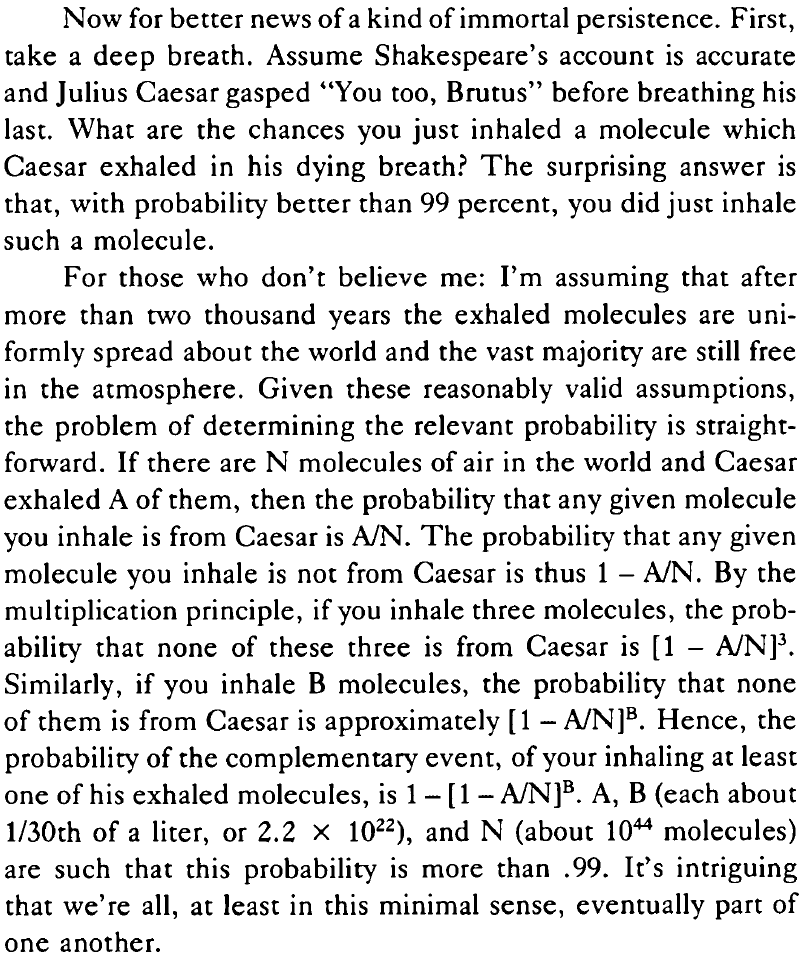
\includegraphics[width=0.6\linewidth]{images/caesar} \end{center}
\end{itemize}

\hypertarget{section-6}{%
\subsection*{61}\label{section-6}}
\addcontentsline{toc}{subsection}{61}

\begin{rmdbox}

\begin{itemize}
\item
  $n$ passageiros para $n$ assentos.
\item
  Passageiro $k$ inicialmente alocado no assento $k$.
\item
  MAS Passageiro $1$ decide escolher assento ao acaso (cada assento com a mesma probabilidade).
\item
  Então, cada passageiro seguinte se senta no assento inicialmente alocado para ele, se disponível; caso contrário, escolhe um assento ao acaso.
\item
  Qual a probabilidade de que o último passageiro se sente no assento alocado para ele?
\end{itemize}

\end{rmdbox}

\hypertarget{possibilidades}{%
\subsubsection*{Possibilidades}\label{possibilidades}}
\addcontentsline{toc}{subsubsection}{Possibilidades}

\begin{itemize}
\item
  O último passageiro só pode se sentar no lugar $1$ ou no lugar $n$.
\item
  Aliás, isto é um caso específico de um fenômeno mais geral: qualquer que seja o valor de $n$:

  \begin{itemize}
  \item
    O passageiro $3$ nunca fica no assento $2$: ou o passageiro $1$ pegou, ou ficou livre para o passageiro $2$ (que é obrigado a pegá-lo).
  \item
    O passageiro $4$ nunca fica nos assentos $2$ nem $3$: ou o passageiro $1$ pegou o assento $3$, ou aconteceu um dos casos acima e o assento $3$ ficou livre para o passageiro $3$ (que é obrigado a pegá-lo).
  \item
    O passageiro $5$ nunca fica nos assentos $2$ nem $3$ nem $4$: ou o passageiro $1$ pegou o assento $4$, ou aconteceu um dos casos acima e o assento $4$ ficou livre para o passageiro $4$ (que é obrigado a pegá-lo).
  \item
    etc.
  \end{itemize}
\item
  Seguindo o raciocínio, chegamos à conclusão de que o passageiro $n$ só pode ocupar o assento $1$ ou o assento $n$.
\end{itemize}

\hypertarget{probabilidades}{%
\subsubsection*{Probabilidades}\label{probabilidades}}
\addcontentsline{toc}{subsubsection}{Probabilidades}

\begin{itemize}
\item
  Examinando exemplos com $n \in \{3, 4, 5\}$, a probabilidade parece ser $1/2$.
\item
  Por quê?
\item
  O assento do passageiro $n$ depende da pergunta (no momento em que o passageiro $n$ vai se sentar)

  {\hl{``O assento $1$ já foi tomado?''}}

  cuja resposta é oposta à da pergunta

  {\hl{``O assento $n$ já foi tomado?''}}
\item
  Com que probabilidade a resposta a esta última pergunta é sim?
\item
  Em todos os passos anteriores, \protect\hyperlink{possibilidades}{como explicado acima em ``possibilidades''}, os assentos $1$ e $n$ sempre estão disponíveis para qualquer passageiro que vá escolher um assento ao acaso.
\item
  Como todos os assentos têm a mesma probabilidade de ser escolhidos, a probabilidade de o assento $1$ estar tomado é igual à probabilidade de o assento $n$ estar tomado.
\item
  Logo, a probabilidade de o passageiro $n$ acabar no assento $n$ é $1/2$.
\end{itemize}

\hypertarget{section-7}{%
\subsection*{62}\label{section-7}}
\addcontentsline{toc}{subsection}{62}

\begin{rmdbox}

\textbf{Problema do aniversário com probabilidades diferentes:}

\begin{itemize}
\item
  Seja $\vec p = (p_1, p_2, \ldots, p_{365})$ o vetor das probabilidades de alguém nascer em algum dos dias do ano.
\item
  Seja

  \[
  e_k(x_1, \ldots, x_n) = 
  \sum_{1 \leq j_1 < j_2 < \cdots < j_k \leq n}
  \!\!\!\!\!\!\!\!\!\!\!\!\!\! x_{j_1} \ldots x_{j_k}
  \]

  o $k$-ésimo {\hl{polinômio simétrico elementar}} sobre as variáveis $x_1, \ldots, x_n$.

  Por exemplo,
  \[
  \begin{aligned}
    e_1(x_1, x_2, x_3) &= x_1 + x_2 + x_3 \\
    e_2(x_1, x_2, x_3) &= x_1x_2 + x_1x_3 + x_2x_3 \\
    e_3(x_1, x_2, x_3) &= x_1x_2x_3 \\
  \end{aligned}
  \]
\end{itemize}

\begin{enumerate}
\def\labelenumi{\alph{enumi}.}
\tightlist
\item
  Seja $k \geq 2$. Qual a probabilidade de pelo menos uma coincidência de aniversários em termos de $\vec p$ e de um polinômio simétrico elementar?
\end{enumerate}

\end{rmdbox}

\begin{itemize}
\item
  A probabilidade de {\hl{não haver coincidência}} é a soma das probabilidades de todos os eventos da forma

  \begin{quote}
  {\hl{As pessoas $1, 2, \ldots k$ nasceram em dias diferentes $j_1, j_2, \ldots, j_k$.}}
  \end{quote}
\item
  Por exemplo, para $k = 3$, a soma será

  \[
  3! \cdot (p_1 p_2 p_3 + p_1 p_2 p_4 + \cdots + p_{363} p_{364} p_{365})
  \]
\item
  Isto é igual a

  \[
  k! \cdot e_k(\vec p)
  \]
\item
  A probabilidade de pelo menos uma coincidência é
  \[
  1 - k! \cdot e_k(\vec p)
  \]
\end{itemize}

\begin{rmdbox}

\begin{enumerate}
\def\labelenumi{\alph{enumi}.}
\setcounter{enumi}{1}
\tightlist
\item
  Quando $p_j = 1/365$ para todo $j$, esta probabilidade é mínima.
\end{enumerate}

\end{rmdbox}

\begin{itemize}
\item
  No caso em que $p_j = p = 1/365$ para todo $j$, temos

  \[
   \begin{aligned}
     1 - k! \cdot e_k(\vec p) 
     &=
     1 - k! \cdot \binom{365}{k} \cdot p^k \\
     &=
     1 - \frac{365 \cdot 364 \cdot \cdots \cdot (365 - k + 1)}{365^k}
   \end{aligned}
   \]
\item
  Neste caso, o valor de $e_k(\vec p)$ é máximo.
\end{itemize}

\begin{rmdbox}

\begin{enumerate}
\def\labelenumi{\alph{enumi}.}
\setcounter{enumi}{2}
\item
  Considere a desigualdade

  \[
  \frac{x + y}{2} \geq \sqrt{xy}
  \]

  que vem do raciocínio

  \[
  \begin{aligned}
    (x + y)^2 - 4xy = (x - y)^2 \geq 0
    \implies &
    (x + y)^2 - 4xy \geq 0
    \\
    \implies &
    (x + y)^2 \geq 4xy
    \\
    \implies &
    \frac{(x + y)^2}{4} \geq xy
    \\
    \implies &
    \frac{x + y}{2} \geq \sqrt{xy}
  \end{aligned}
  \]

  Defina $\vec r = (r_1, \ldots, r_{365})$ tal que

  \begin{itemize}
  \item
    $r_1 = r_2 = (p_1 + p_2)/2$,
  \item
    $r_j = p_j$ para $3 \leq j \leq 365$.
  \end{itemize}

  Verifique que
  \[
  \begin{aligned}
    e_k(x_1, \ldots, x_n)
    &=
    x_1 x_2 e_{k-2}(x_3, \ldots x_n) \;+ \\
    &\phantom{{}={}} (x_1 + x_2) e_{k-1}(x_3, \ldots x_n) \;+ \\
    &\phantom{{}={}} e_{k}(x_3, \ldots x_n)
  \end{aligned}
  \]

  e use a desigualdade para mostrar que, quando $\vec p \neq \vec r$,

  \[
  P( \text{coincidência} \mid \vec p) 
  >
  P( \text{coincidência} \mid \vec r)
  \]
\end{enumerate}

\end{rmdbox}

\begin{itemize}
\item
  Observe que

  \[
  \frac{x + y}{2} = \sqrt{xy} \implies x = y
  \]

  Ou seja, quando $x \neq y$, a desigualdade é estrita.
\item
  Para o vetor $\vec p$:

  \[
  \begin{aligned}
  &
  P( \text{coincidência} \mid \vec p) \\
  &=
  1 - k! \cdot e_k(\vec p) \\
  &=
  1 - k! \cdot \left[ 
  p_1p_2 \cdot e_{k-2}(p_3, \ldots p_n) +
  (p_1 + p_2) \cdot e_{k-1}(p_3, \ldots p_n) +
  e_{k}(p_3, \ldots p_n)
  \right]
  \end{aligned}
  \]
\item
  Para o vetor $\vec r$:

  \[
  \begin{aligned}
  &
  P( \text{coincidência} \mid \vec r) \\
  &=
  1 - k! \cdot e_k(\vec r) \\
  &=
  1 - k! \cdot \left[ 
  \frac{(p_1 + p_2)^2}{4} \cdot e_{k-2}(p_3, \ldots p_n) +
  (p_1 + p_2) \cdot e_{k-1}(p_3, \ldots p_n) +
  e_{k}(p_3, \ldots p_n)
  \right]
  \end{aligned}
  \]
\item
  A única diferença está no primeiro fator dentro dos colchetes.
\item
  Pela desigualdade:

  \[
  \frac{p_1 + p_2}{2} \geq \sqrt{p_1p_2} \implies 
  \frac{(p_1 + p_2)^2}{4} \geq p_1p_2
  \]
\item
  Conclusão: para todo vetor $\vec p$ de probabilidades, é possível preservar ou diminuir a probabilidade de uma coincidência substituindo quaisquer $2$ de suas componentes pelo valor da média aritmética delas. Assim, o vetor que minimiza a probabilidade precisa ter todas as suas componentes iguais.
\end{itemize}

\hypertarget{probabilidade-condicional}{%
\chapter*{04: Probabilidade condicional}\label{probabilidade-condicional}}
\addcontentsline{toc}{chapter}{04: Probabilidade condicional}

\hypertarget{vuxeddeo-3}{%
\section*{Vídeo}\label{vuxeddeo-3}}
\addcontentsline{toc}{section}{Vídeo}

\begin{center} \url{https://youtu.be/P7NE4WF8j-Q} \end{center}

\hypertarget{exercuxedcios-do-livro-cap.-2}{%
\section*{Exercícios do livro (cap. 2)}\label{exercuxedcios-do-livro-cap.-2}}
\addcontentsline{toc}{section}{Exercícios do livro (cap. 2)}

\hypertarget{section-8}{%
\subsection*{2}\label{section-8}}
\addcontentsline{toc}{subsection}{2}

\begin{rmdbox}

\begin{itemize}
\item
  Uma mulher está grávida de meninos gêmeos.
\item
  Gêmeos podem ser idênticos ou fraternos.
\item
  $1/3$ dos gêmeos são idênticos.
\item
  Gêmeos idênticos têm $50\%$ de chance de serem ambos meninos, e $50\%$ de chance de serem ambos meninas.
\item
  Para gêmeos fraternos, cada gêmeo tem, independentemente, $50\%$ de chance de ser menino, e $50\%$ de chance de ser menina.
\item
  Qual a probabilidade de a mulher estar grávida de gêmeos idênticos?
\end{itemize}

\end{rmdbox}

\begin{itemize}
\item
  Eventos:

  \[
  \begin{aligned}
  I &= \text{os gêmeos são idênticos} \\
  M &= \text{os gêmeos são dois meninos}
  \end{aligned}
  \]
\item
  Probabilidades dadas:

  \[
  \begin{aligned}
  P(I) &= 1/3 \\
  P(M \mid I) &= 1/2 \\
  P(M \mid \neg I) &= 1/4
  \end{aligned}
  \]
\item
  Queremos calcular $P(I \mid M)$. Usamos Bayes:

  \[
  \begin{aligned}
  P(I \mid M) 
  &=
  \frac{P(M \mid I) \cdot P(I)}{P(M)}
  \end{aligned}
  \]
\item
  Só falta o valor de $P(M)$, que calculamos usando probabilidade total:

  \[
  \begin{aligned}
  P(M) 
  &=
  P(M \mid I)P(I) + P(M \mid \neg I)P(\neg I) \\
  &=
  1/2 \cdot 1/3 + 1/4 \cdot 2/3 \\
  &=
  1/3
  \end{aligned}
  \]
\item
  Concluímos

  \[
  \begin{aligned}
  P(I \mid M) 
  &=
  \frac{P(M \mid I) \cdot P(I)}{P(M)} \\
  &=
  \frac{1/2 \cdot 1/3}{1/3} \\
  &=
  1/2
  \end{aligned}
  \]
\end{itemize}

\hypertarget{section-9}{%
\subsection*{4}\label{section-9}}
\addcontentsline{toc}{subsection}{4}

\begin{rmdbox}

\begin{itemize}
\item
  Um aluno está resolvendo uma questão de múltipla escolha com $n$ opções.
\item
  $K$ é o evento que corresponde a ele saber a resposta correta.
\item
  $R$ é o evento que corresponde a ele acertar (sabendo ou chutando).
\item
  Se ele sabe a resposta, ele acerta.
\item
  Se ele não sabe, ele chuta uma opção ao acaso.
\item
  Considere $P(K) = p$.
\end{itemize}

\begin{enumerate}
\def\labelenumi{(\alph{enumi})}
\item
  Ache $P(K \mid R)$.
\item
  Mostre que $P(K \mid R) \geq p$. Por que isto faz sentido? Quando a igualdade é exata?
\end{enumerate}

\end{rmdbox}

\begin{enumerate}
\def\labelenumi{\alph{enumi}.}
\item
  Vamos usar Bayes, supondo $p = P(K) > 0$:

  \[
  \begin{aligned}
  P(K \mid R)
  &=
  \frac{P(R \mid K) \cdot P(K)}{P(R)} \\
  &=
  \frac{1 \cdot p}{
    P(R \mid K) \cdot P(K) + 
    P(R \mid \neg K) \cdot P(\neg K)
  } \\
  &=
  \frac{p}{
    1 \cdot p + 
    \frac{1}{n} \cdot (1 - p)
  } \\
  &=
  \frac{np}{np + (1 - p)}
  \end{aligned}
  \]
\item
  Isto equivale a mostrar

  \[
  \frac{np}{np + (1 - p)} \geq p
  \]

  Como todos os valores são positivos, isto equivale a

  \[
  np \geq np^2 + (1 - p)p
  \]

  Dividindo ambos os lados por $p > 0$:

  \[
  n \geq np + 1 - p
  \]

  Daí,

  \[
  \begin{aligned}
  n \geq np + 1 - p 
  &\iff n - np \geq 1 - p \\
  &\iff n(1 - p) \geq 1 - p \\
  &\iff n \geq 1 & \text{(supondo } p < 1 \text{)}
  \end{aligned}
  \]
  O que é verdade, pois existe pelo menos uma opção (a correta).

  Se $p = 1$, a igualdade vale, e $P(K \mid R) = 1$, pois o aluno sempre sabe a resposta e sempre acerta.

  Se $n = 1$, a igualdade vale, e $P(K \mid R) = p$, pois o aluno acertar (ele sempre acerta!) e o aluno saber são independentes.

  Imagine $n > 1$.

  Lembre-se de que $P(K \mid R) = \frac{P(K \cap R)}{P(R)}$.

  O numerador é a probabilidade do evento ``o aluno sabe e o aluno acerta''. Esta probabilidade é exatamente $p$, pois ``o aluno sabe'' é sub-evento de ``o aluno acerta''.

  O numerador $P(R)$ é um número tal que $0 < P(R) < 1$. Vamos chamar este número de $1/x$, para $x > 1$.

  Então,

  \[
  P(K \mid R) = \frac{P(K \cap R)}{P(R)} = \frac{p}{1/x} = xp > p
  \]
\end{enumerate}

\hypertarget{em-r}{%
\subsubsection*{Em R}\label{em-r}}
\addcontentsline{toc}{subsubsection}{Em R}

Valores teóricos:

\begin{Shaded}
\begin{Highlighting}[]
\NormalTok{n }\OtherTok{\textless{}{-}} \DecValTok{1}\SpecialCharTok{:}\DecValTok{9}
\NormalTok{p }\OtherTok{\textless{}{-}} \FunctionTok{seq}\NormalTok{(}\DecValTok{0}\NormalTok{, }\DecValTok{1}\NormalTok{, .}\DecValTok{25}\NormalTok{)}

\NormalTok{df }\OtherTok{\textless{}{-}} \FunctionTok{expand.grid}\NormalTok{(}\AttributeTok{n =}\NormalTok{ n, }\AttributeTok{p =}\NormalTok{ p) }\SpecialCharTok{\%\textgreater{}\%} 
  \FunctionTok{mutate}\NormalTok{(}
    \AttributeTok{pkr\_teorico =}\NormalTok{ n }\SpecialCharTok{*}\NormalTok{ p }\SpecialCharTok{/}\NormalTok{ (p }\SpecialCharTok{*}\NormalTok{ (n }\SpecialCharTok{{-}} \DecValTok{1}\NormalTok{) }\SpecialCharTok{+} \DecValTok{1}\NormalTok{)}
\NormalTok{  ) }\SpecialCharTok{\%\textgreater{}\%} 
  \FunctionTok{arrange}\NormalTok{(n)}

\NormalTok{df}
\DocumentationTok{\#\# \# A tibble: 45 x 3}
\DocumentationTok{\#\#       n     p pkr\_teorico}
\DocumentationTok{\#\#   \textless{}int\textgreater{} \textless{}dbl\textgreater{}       \textless{}dbl\textgreater{}}
\DocumentationTok{\#\# 1     1  0           0   }
\DocumentationTok{\#\# 2     1  0.25        0.25}
\DocumentationTok{\#\# 3     1  0.5         0.5 }
\DocumentationTok{\#\# 4     1  0.75        0.75}
\DocumentationTok{\#\# 5     1  1           1   }
\DocumentationTok{\#\# 6     2  0           0   }
\DocumentationTok{\#\# \# ... with 39 more rows}
\end{Highlighting}
\end{Shaded}

Gráfico:

\begin{center}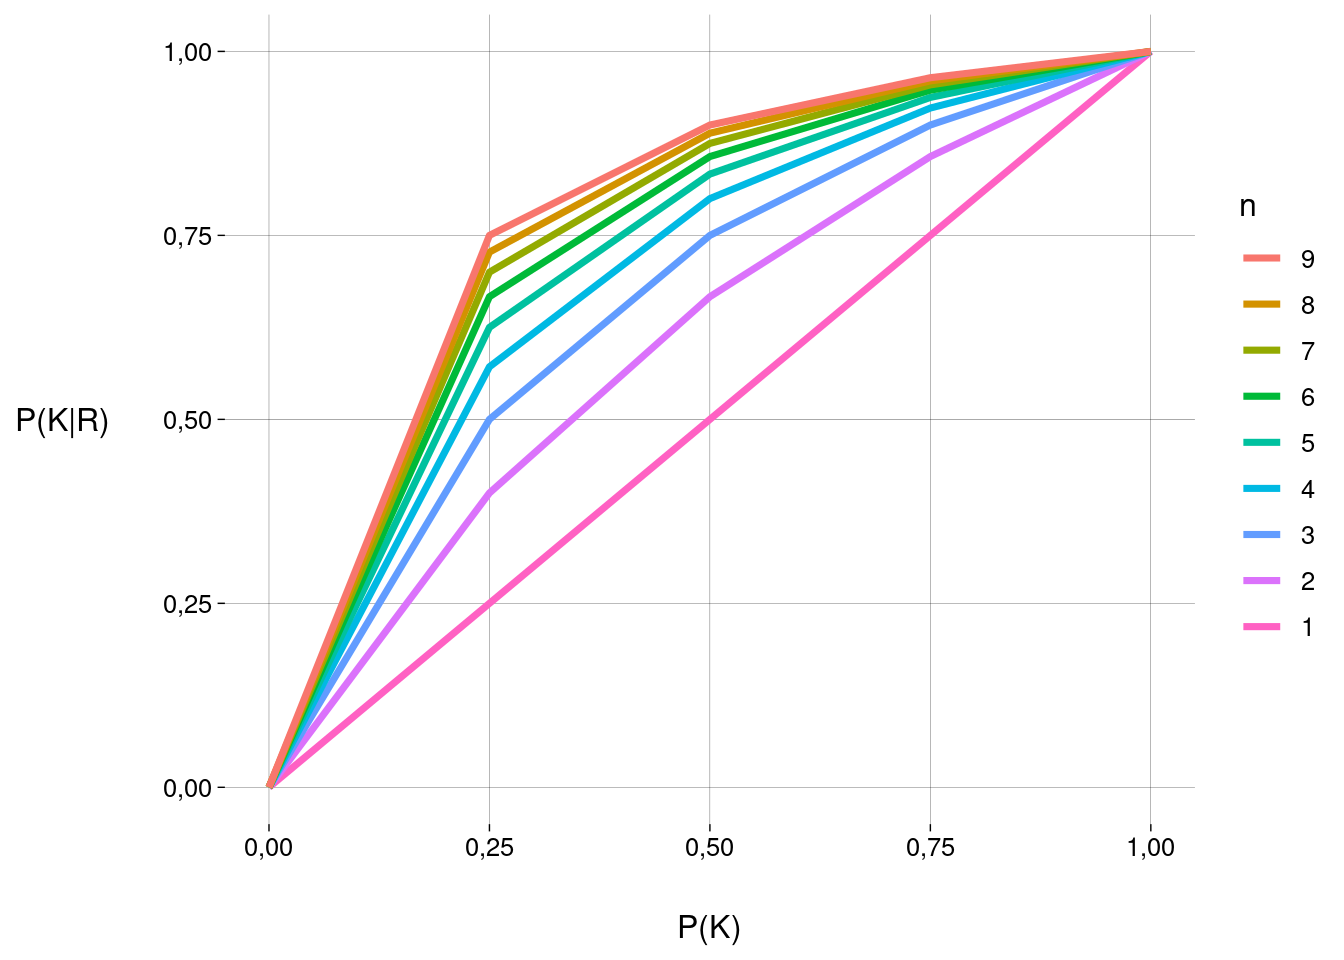
\includegraphics[width=1\linewidth]{_main_files/figure-latex/unnamed-chunk-24-1} \end{center}

\begin{rmdnote}
Conclusão óbvia: quanto maior o número $n$ de opções, maior a probabilidade $P(K \mid R)$ de o aluno ter acertado sabendo, em oposição a ter acertado chutando:

\[
\begin{aligned}
\lim_{n \to \infty} P(K \mid R) 
&=
\lim_{n \to \infty} \frac{np}{np + 1 - p} \\
&=
\lim_{n \to \infty} \frac{p}{p} \\
&= 1
\end{aligned}
\]

\end{rmdnote}

Simulação:

\begin{Shaded}
\begin{Highlighting}[]
\NormalTok{sim }\OtherTok{\textless{}{-}} \ControlFlowTok{function}\NormalTok{(n, p, }\AttributeTok{reps =} \FloatTok{1e7}\NormalTok{) \{}
  
\NormalTok{  sabe }\OtherTok{\textless{}{-}} \FunctionTok{sample}\NormalTok{(}
    \FunctionTok{c}\NormalTok{(}\ConstantTok{TRUE}\NormalTok{, }\ConstantTok{FALSE}\NormalTok{), }
\NormalTok{    reps,}
    \AttributeTok{replace =} \ConstantTok{TRUE}\NormalTok{,}
    \FunctionTok{c}\NormalTok{(p, }\DecValTok{1} \SpecialCharTok{{-}}\NormalTok{ p)}
\NormalTok{  )}

\NormalTok{  acerta }\OtherTok{\textless{}{-}}\NormalTok{ sabe}
\NormalTok{  nao\_sabe }\OtherTok{\textless{}{-}} \FunctionTok{sum}\NormalTok{(}\SpecialCharTok{!}\NormalTok{sabe)}
  
\NormalTok{  acerta[}\FunctionTok{which}\NormalTok{(}\SpecialCharTok{!}\NormalTok{sabe)] }\OtherTok{\textless{}{-}} 
    \FunctionTok{sample}\NormalTok{(}
      \FunctionTok{c}\NormalTok{(}\ConstantTok{TRUE}\NormalTok{, }\ConstantTok{FALSE}\NormalTok{),}
\NormalTok{      nao\_sabe,}
      \AttributeTok{replace =} \ConstantTok{TRUE}\NormalTok{,}
      \AttributeTok{prob =} \FunctionTok{c}\NormalTok{(}\DecValTok{1}\SpecialCharTok{/}\NormalTok{n, }\DecValTok{1} \SpecialCharTok{{-}} \DecValTok{1}\SpecialCharTok{/}\NormalTok{n)}
\NormalTok{    )}
  
  \FunctionTok{sum}\NormalTok{(sabe) }\SpecialCharTok{/} \FunctionTok{sum}\NormalTok{(acerta)}
  
\NormalTok{\}}

\NormalTok{sim }\OtherTok{\textless{}{-}} \FunctionTok{Vectorize}\NormalTok{(sim)}
\end{Highlighting}
\end{Shaded}

\begin{Shaded}
\begin{Highlighting}[]
\NormalTok{df }\OtherTok{\textless{}{-}}\NormalTok{ df }\SpecialCharTok{\%\textgreater{}\%} 
  \FunctionTok{mutate}\NormalTok{(}
    \AttributeTok{pkr\_simulado =} \FunctionTok{sim}\NormalTok{(n, p)}
\NormalTok{  )}

\NormalTok{df}
\DocumentationTok{\#\# \# A tibble: 45 x 4}
\DocumentationTok{\#\#       n     p pkr\_teorico pkr\_simulado}
\DocumentationTok{\#\#   \textless{}int\textgreater{} \textless{}dbl\textgreater{}       \textless{}dbl\textgreater{}        \textless{}dbl\textgreater{}}
\DocumentationTok{\#\# 1     1  0           0           0    }
\DocumentationTok{\#\# 2     1  0.25        0.25        0.250}
\DocumentationTok{\#\# 3     1  0.5         0.5         0.500}
\DocumentationTok{\#\# 4     1  0.75        0.75        0.750}
\DocumentationTok{\#\# 5     1  1           1           1    }
\DocumentationTok{\#\# 6     2  0           0           0    }
\DocumentationTok{\#\# \# ... with 39 more rows}
\end{Highlighting}
\end{Shaded}

\begin{center}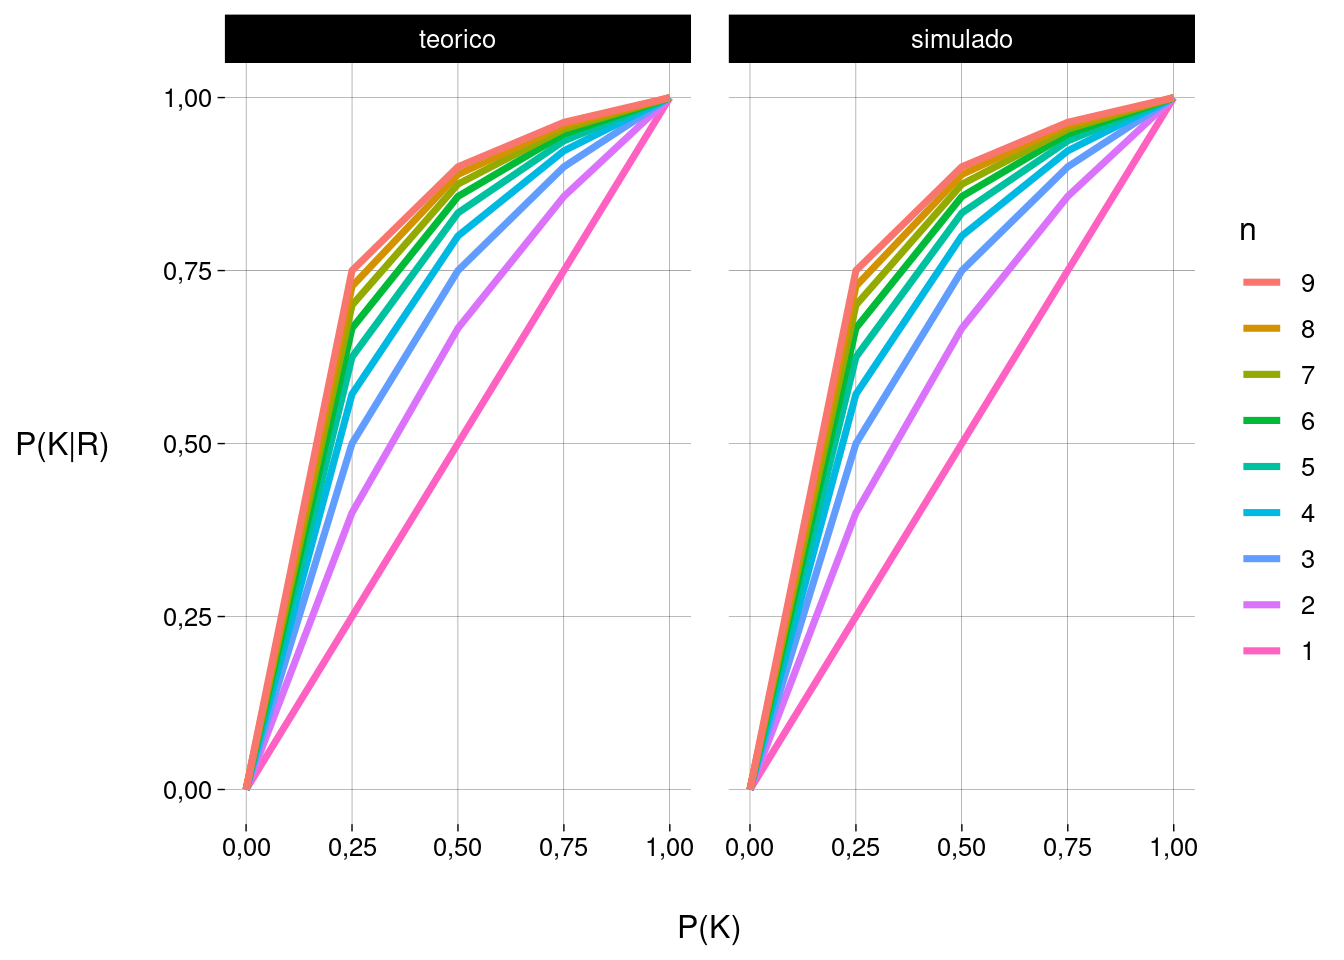
\includegraphics[width=1\linewidth]{_main_files/figure-latex/unnamed-chunk-27-1} \end{center}

\hypertarget{section-10}{%
\subsection*{12}\label{section-10}}
\addcontentsline{toc}{subsection}{12}

\begin{rmdbox}

\begin{enumerate}
\def\labelenumi{\alph{enumi}.}
\item
  Alice está tentando enviar uma mensagem codificada em binário para Bob.

  \begin{itemize}
  \item
    Ela envia um \emph{bit}: $0$ ou $1$ com probabilidades iguais.
  \item
    Se ela envia $0$, há probabilidade $5\%$ de erro.
  \item
    Se ela envia $1$, há probabilidade $10\%$ de erro.
  \item
    Dado que Bob recebeu $1$, qual a probabilidade de Alice ter enviado $1$?
  \end{itemize}
\end{enumerate}

\end{rmdbox}

\begin{itemize}
\item
  Eventos e probabilidades:

  \begin{center}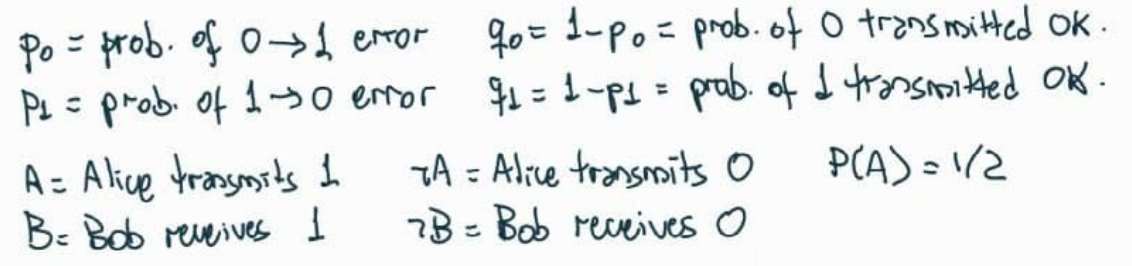
\includegraphics[width=1\linewidth]{images/alice01} \end{center}
\item
  Queremos achar $P(A \mid B)$. Usando Bayes:

  \begin{center}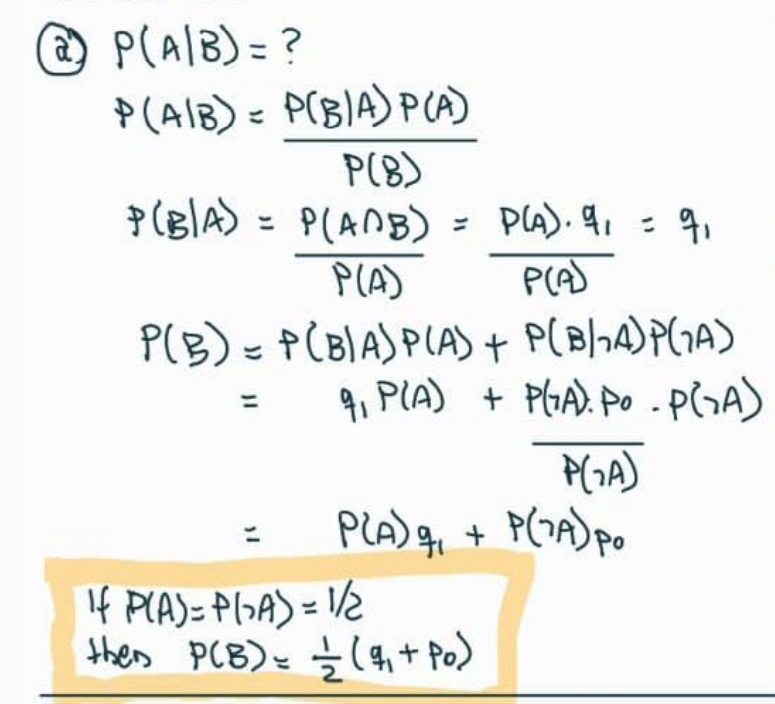
\includegraphics[width=0.75\linewidth]{images/alice02} \end{center}

\begin{Shaded}
\begin{Highlighting}[]
\NormalTok{p0 }\OtherTok{\textless{}{-}}\NormalTok{ .}\DecValTok{05}
\NormalTok{p1 }\OtherTok{\textless{}{-}}\NormalTok{ .}\DecValTok{1}
\NormalTok{q0 }\OtherTok{\textless{}{-}} \DecValTok{1} \SpecialCharTok{{-}}\NormalTok{ p0}
\NormalTok{q1 }\OtherTok{\textless{}{-}} \DecValTok{1} \SpecialCharTok{{-}}\NormalTok{ p1}

\NormalTok{pA }\OtherTok{\textless{}{-}} \DecValTok{1}\SpecialCharTok{/}\DecValTok{2}
\NormalTok{pBIA }\OtherTok{\textless{}{-}}\NormalTok{ q1}
\NormalTok{pB }\OtherTok{\textless{}{-}}\NormalTok{ (q1 }\SpecialCharTok{+}\NormalTok{ p0) }\SpecialCharTok{/} \DecValTok{2}
\NormalTok{pAIB }\OtherTok{\textless{}{-}}\NormalTok{ pBIA }\SpecialCharTok{*}\NormalTok{ pA }\SpecialCharTok{/}\NormalTok{ pB}

\NormalTok{pAIB}
\DocumentationTok{\#\# [1] 0,9473684}
\end{Highlighting}
\end{Shaded}
\item
  Para sermos completos, vamos calcular outras probabilidades, com $P(A) = P(\neg A) = 1/2$:

  \begin{center}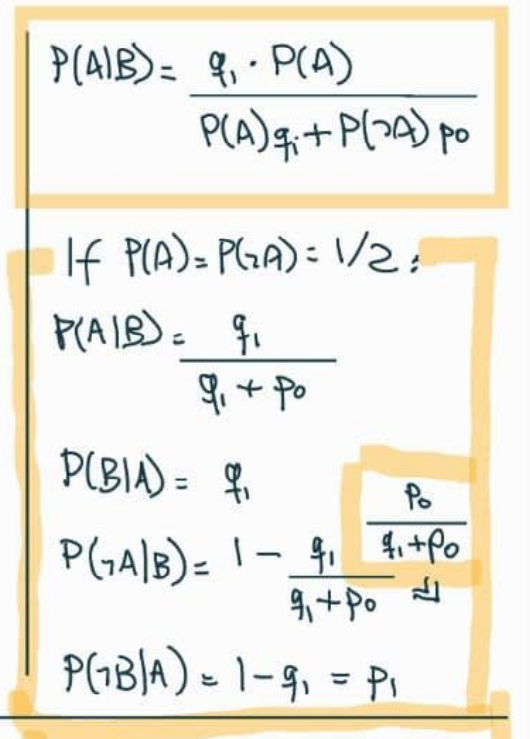
\includegraphics[width=0.5\linewidth]{images/alice03} \end{center}

  \begin{center}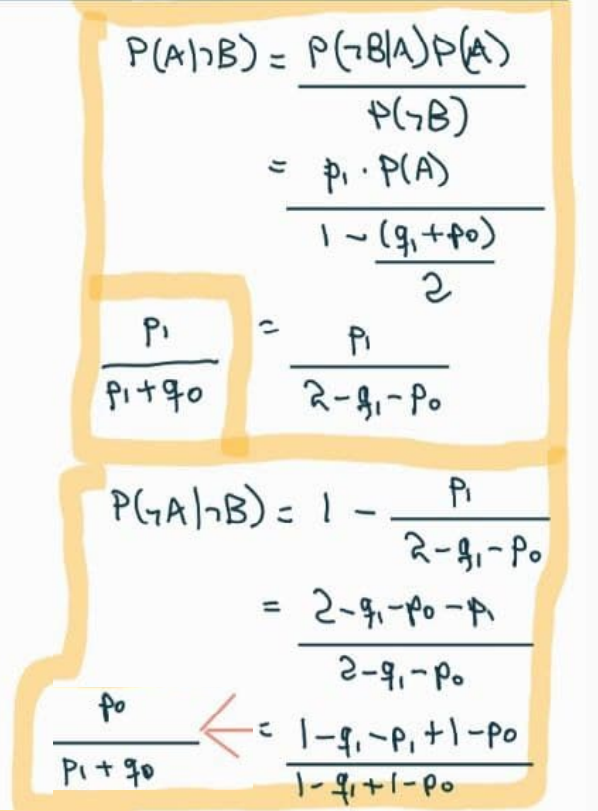
\includegraphics[width=0.5\linewidth]{images/alice04} \end{center}
\item
  Simulação:

\begin{Shaded}
\begin{Highlighting}[]
\NormalTok{reps }\OtherTok{\textless{}{-}} \FloatTok{1e7}
\NormalTok{alice\_envia }\OtherTok{\textless{}{-}} \FunctionTok{sample}\NormalTok{(}\FunctionTok{c}\NormalTok{(}\DecValTok{0}\NormalTok{, }\DecValTok{1}\NormalTok{), reps, }\AttributeTok{replace =} \ConstantTok{TRUE}\NormalTok{)}
\NormalTok{bob\_recebe }\OtherTok{\textless{}{-}}\NormalTok{ alice\_envia}

\NormalTok{bob\_recebe[}\FunctionTok{which}\NormalTok{(alice\_envia }\SpecialCharTok{==} \DecValTok{0}\NormalTok{)] }\OtherTok{\textless{}{-}} 
  \FunctionTok{sample}\NormalTok{(}
    \FunctionTok{c}\NormalTok{(}\DecValTok{0}\NormalTok{, }\DecValTok{1}\NormalTok{), }
    \FunctionTok{length}\NormalTok{(}\FunctionTok{which}\NormalTok{(alice\_envia }\SpecialCharTok{==} \DecValTok{0}\NormalTok{)),}
    \AttributeTok{replace =} \ConstantTok{TRUE}\NormalTok{,}
    \AttributeTok{prob =} \FunctionTok{c}\NormalTok{(}\DecValTok{95}\SpecialCharTok{/}\DecValTok{100}\NormalTok{, }\DecValTok{5}\SpecialCharTok{/}\DecValTok{100}\NormalTok{)}
\NormalTok{  )}

\NormalTok{bob\_recebe[}\FunctionTok{which}\NormalTok{(alice\_envia }\SpecialCharTok{==} \DecValTok{1}\NormalTok{)] }\OtherTok{\textless{}{-}} 
  \FunctionTok{sample}\NormalTok{(}
    \FunctionTok{c}\NormalTok{(}\DecValTok{0}\NormalTok{, }\DecValTok{1}\NormalTok{), }
    \FunctionTok{length}\NormalTok{(}\FunctionTok{which}\NormalTok{(alice\_envia }\SpecialCharTok{==} \DecValTok{1}\NormalTok{)),}
    \AttributeTok{replace =} \ConstantTok{TRUE}\NormalTok{,}
    \CommentTok{\# Atenção: aqui, erro é 1 virar 0:}
    \AttributeTok{prob =} \FunctionTok{c}\NormalTok{(}\DecValTok{10}\SpecialCharTok{/}\DecValTok{100}\NormalTok{, }\DecValTok{90}\SpecialCharTok{/}\DecValTok{100}\NormalTok{)  }
\NormalTok{  )}

\NormalTok{pab }\OtherTok{\textless{}{-}} \FunctionTok{sum}\NormalTok{(alice\_envia }\SpecialCharTok{\&}\NormalTok{ bob\_recebe) }\SpecialCharTok{/} \FunctionTok{sum}\NormalTok{(bob\_recebe)}
\NormalTok{pab}
\DocumentationTok{\#\# [1] 0,9473928}
\end{Highlighting}
\end{Shaded}
\end{itemize}

\begin{rmdbox}

\begin{enumerate}
\def\labelenumi{\alph{enumi}.}
\setcounter{enumi}{1}
\item
  Agora, eles usam um {\hl{código com repetição}}:

  \begin{itemize}
  \item
    Alice envia $000$ para representar $0$ e $111$ para representar $1$.
  \item
    Bob decodifica a mensagem tomando o \emph{bit} que está em maioria.
  \item
    As probabilidades de erro são como antes, e os erros em \emph{bits} diferentes são independentes.
  \item
    Dado que Bob recebe $110$, qual a probabilidade de que Alice tenha enviado $111$?
  \end{itemize}
\end{enumerate}

\end{rmdbox}

\begin{itemize}
\item
  Eventos:

  \[
  \begin{aligned}
  AAA &= \text{Alice envia } 111 \\
  BB\neg B &= \text{Bob recebe } 110
  \end{aligned}
  \]
\item
  $P(AAA) = 1/2$, pois Alice envia somente $111$ ou $000$.
\item
  Usando Bayes:

  \[
  P(AAA \mid BB\neg B) = 
  \frac{P(BB\neg B \mid AAA) \cdot P(AAA)}{P(BB\neg B)}
  \]
\item
  $P(BB\neg B \mid AAA) = q_1 \cdot q_1 \cdot p_1$, pois erros em \emph{bits} diferentes são independentes.
\item
  Pela lei da probabilidade total:

  \[
  \begin{aligned}
  P(BB\neg B) 
  &= P(BB\neg B \mid AAA) \cdot P(AAA) + 
     P(BB\neg B \mid \neg(AAA))P(\neg(AAA)) \\
  &= \frac12 \cdot \left( q_1 \cdot q_1 \cdot p_1 +
     p_0 \cdot p_0 \cdot q_0 \right)
  \end{aligned}
  \]
\item
  Daí,

  \[
  \begin{aligned}
  P(AAA \mid BB\neg B) 
  &= 
  \frac{P(BB\neg B \mid AAA) \cdot P(AAA)}{P(BB\neg B)} \\
  &= 
  \frac{
    q_1 \cdot q_1 \cdot p_1 \cdot 1/2
  }{
    \left( q_1 \cdot q_1 \cdot p_1 +
     p_0 \cdot p_0 \cdot q_0 \right)\cdot 1/2
  } \\
  &= 
  \frac{
    q_1 \cdot q_1 \cdot p_1
  }{
    \left( q_1 \cdot q_1 \cdot p_1 +
     p_0 \cdot p_0 \cdot q_0 \right)
  }
  \end{aligned}
  \]
\item
  Numericamente:

\begin{Shaded}
\begin{Highlighting}[]
\NormalTok{q1 }\SpecialCharTok{*}\NormalTok{ q1 }\SpecialCharTok{*}\NormalTok{ p1 }\SpecialCharTok{/}\NormalTok{ (q1 }\SpecialCharTok{*}\NormalTok{ q1 }\SpecialCharTok{*}\NormalTok{ p1 }\SpecialCharTok{+}\NormalTok{ p0 }\SpecialCharTok{*}\NormalTok{ p0 }\SpecialCharTok{*}\NormalTok{ q0)}
\DocumentationTok{\#\# [1] 0,9715142}
\end{Highlighting}
\end{Shaded}
\end{itemize}

\hypertarget{section-11}{%
\subsection*{14}\label{section-11}}
\addcontentsline{toc}{subsection}{14}

\begin{rmdbox}
Se $P(A), P(B) \in (0, 1)$, então

\[
P(A \mid B) > P(A \mid \neg B) \iff
P(B \mid A) > P(B \mid \neg A)
\]

\end{rmdbox}

???

\hypertarget{section-12}{%
\subsection*{15}\label{section-12}}
\addcontentsline{toc}{subsection}{15}

\begin{rmdbox}

$A$ e $B$ são eventos com

\[
0 < P(A \cap B) < P(A) < P(B) < P(A \cup B) < 1
\]

Você está torcendo para que $A$ e $B$ {\hl{ambos}} ocorram.

O que você ficaria mais feliz em observar?

\begin{itemize}
\item
  Que $A$ ocorreu?
\item
  Que $B$ ocorreu?
\item
  Que $A \cup B$ ocorreu?
\end{itemize}

\end{rmdbox}

\begin{itemize}
\item
  Queremos observar o evento $E$ tal que $P(A \cap B \mid E)$ seja máximo.

  \[
  \begin{aligned}
  P(A \cap B \mid A) &= \frac{P(A \cap B)}{P(A)} \\
  P(A \cap B \mid B) &= \frac{P(A \cap B)}{P(B)} \\
  P(A \cap B \mid A \cup B) &= 
    \frac{P((A \cap B) \cap (A \cup B))}{P(A \cup B)} \\
    &= \frac{P(A \cap B)}{P(A \cup B)}
  \end{aligned}
  \]
\item
  Como $P(A)$ é o menor denominador, observar $A$ maximiza $P(A \cap B \mid E)$.
\item
  Intuitivamente, como $A$ é o evento menos provável dos dois, saber que $A$ ocorreu nos deixa mais próximo da ocorrência dos dois eventos do que saber que $B$ (ou que algum dos dois) ocorreu.
\end{itemize}

\hypertarget{section-13}{%
\subsection*{16}\label{section-13}}
\addcontentsline{toc}{subsection}{16}

\begin{rmdbox}
\[
P(A \mid B) \leq P(A) \implies P(A \mid \neg B) \geq P(A)
\]

\end{rmdbox}

\begin{itemize}
\item
  Se a ocorrência de $B$ torna $A$ menos provável, então a não-ocorrência de $B$ torna $A$ mais provável.
\item
  Pela lei da probabilidade total:

  \[
  \begin{aligned}
  P(A) &= P(A \mid B)P(B) + P(A \mid \neg B)P(\neg B) \\
  \therefore P(A \mid \neg B) &= 
    \frac{P(A) - P(A \mid B)P(B)}{P(\neg B)}
  \end{aligned}
  \]
\item
  Daí,

  \[
  \begin{aligned}
  P(A \mid \neg B) 
  &\geq
    \frac{P(A) - P(A)P(B)}{P(\neg B)} & \text{pois } P(A \mid B) \leq P(A) \\
  &= \frac{P(A)(1 - P(B))}{P(\neg B)} \\
  &= P(A)
  \end{aligned}
  \]
\end{itemize}

\hypertarget{section-14}{%
\subsection*{17}\label{section-14}}
\addcontentsline{toc}{subsection}{17}

\begin{rmdbox}

Em lógica determinística, $A \to B \iff \neg B \to \neg A$.

Em probabilidades?

Considere eventos $A$ e $B$ com $P(A), P(B) \not\in \{0, 1\}$.

\begin{enumerate}
\def\labelenumi{\alph{enumi}.}
\tightlist
\item
  Mostre que $P(B \mid A) = 1 \implies P(\neg A \mid \neg B) = 1$.
\end{enumerate}

\end{rmdbox}

\begin{itemize}
\item
  $A$ está contido em $B$:

  \[
  P(B \mid A) = 1 
  \iff \frac{P(A \cap B)}{P(A)} = 1
  \iff P(A \cap B) = P(A)
  \]
\item
  Vamos mostrar que $P(\neg A \mid \neg B) = 1$:

  \[
  \begin{aligned}
  P(\neg A \mid \neg B) 
  &= \frac{P(\neg A \cap \neg B)}{P(\neg B)} \\
  &= \frac{P(\neg (A \cup B))}{P(\neg B)} \\
  &= \frac{1 - P(A \cup B)}{P(\neg B)} \\
  &= \frac{1 - \left[ P(A) + P(B) - P(A \cap B) \right]}{P(\neg B)} \\
  &= \frac{1 - P(B)}{P(\neg B)} \\
  &= \frac{P(\neg B)}{P(\neg B)} \\
  &= 1
  \end{aligned}
  \]
\end{itemize}

\begin{rmdbox}

\begin{enumerate}
\def\labelenumi{\alph{enumi}.}
\setcounter{enumi}{1}
\tightlist
\item
  Mostre que, se ``$=$'' for substituído por ``$\approx$'', o resultado não vale. Ache um exemplo em que $P(B \mid A)$ seja quase $1$, mas $P(\neg A \mid \neg B)$ seja quase $0$.
\end{enumerate}

\end{rmdbox}

\begin{itemize}
\item
  Valores de exemplo, com $A$ e $B$ independentes:

  \[
  \begin{aligned}
  P(A) &= 80/100 \\
  P(B) &= 90/100 \\
  P(\neg A) &= 20/100 \\
  P(\neg B) &= 10/100 \\
  P(A \cap B) &= P(A) \cdot P(B) = 72/100 \\
  P(A \cup B) &= P(A) + P(B) - P(A \cap B) = 98/100\\
  P(B \mid A) &= \frac{P(A \cap B)}{P(A)} = 72/80 \approx 1 \\
  P(\neg A \mid \neg B) &= \frac{P(\neg A \cap \neg B)}{P(\neg B)} = 
    \frac{1 - P(A \cup B)}{P(\neg B)} = 2/10 \approx 0
  \end{aligned}
  \]
\end{itemize}

\hypertarget{i}{}
\begin{rmdnote}

Vamos criar uma medida de independência. Se $P(A) \neq 0$ e $P(B) \neq 0$, definimos

\[
I = \frac{P(A \cap B)}{P(A)P(B)}
\]

Com isso,

\begin{itemize}
\item
  $A$ e $B$ são disjuntos ${} \iff I = 0$
\item
  $A$ e $B$ são independentes ${} \iff I = 1$
\item
  $A$ e $B$ se atrapalham ${} \iff 0 < I < 1$.

  I.e., $P(A) > P(A \mid B)$ e $P(B) > P(B \mid A)$.
\item
  $A$ e $B$ se ajudam ${} \iff I > 1$.

  I.e., $P(A) < P(A \mid B)$ e $P(B) < P(B \mid A)$.
\end{itemize}

\end{rmdnote}

\begin{center}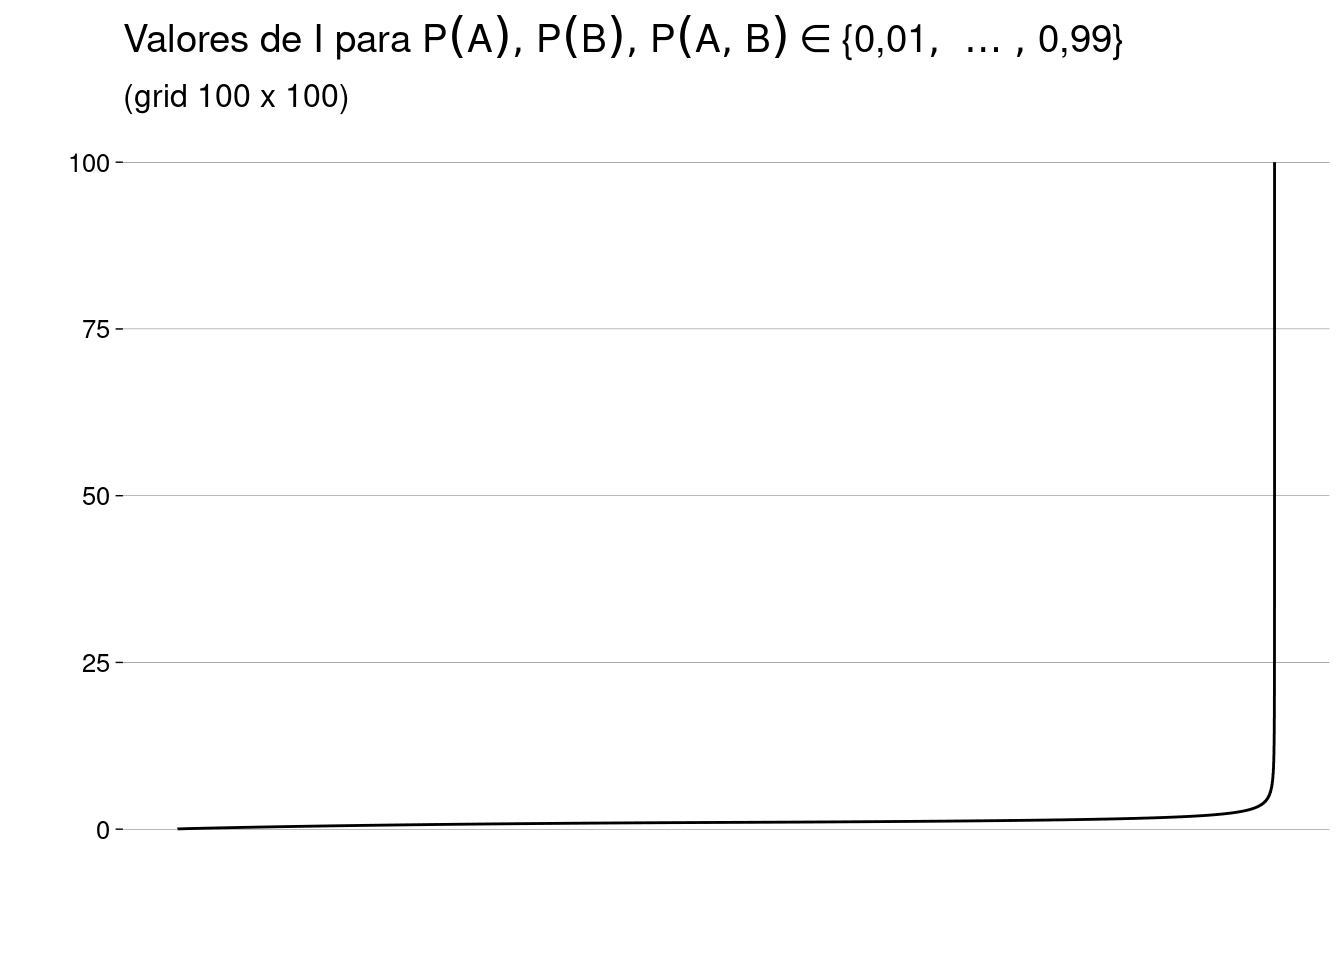
\includegraphics[width=1\linewidth]{_main_files/figure-latex/unnamed-chunk-35-1} \end{center}

\begin{center}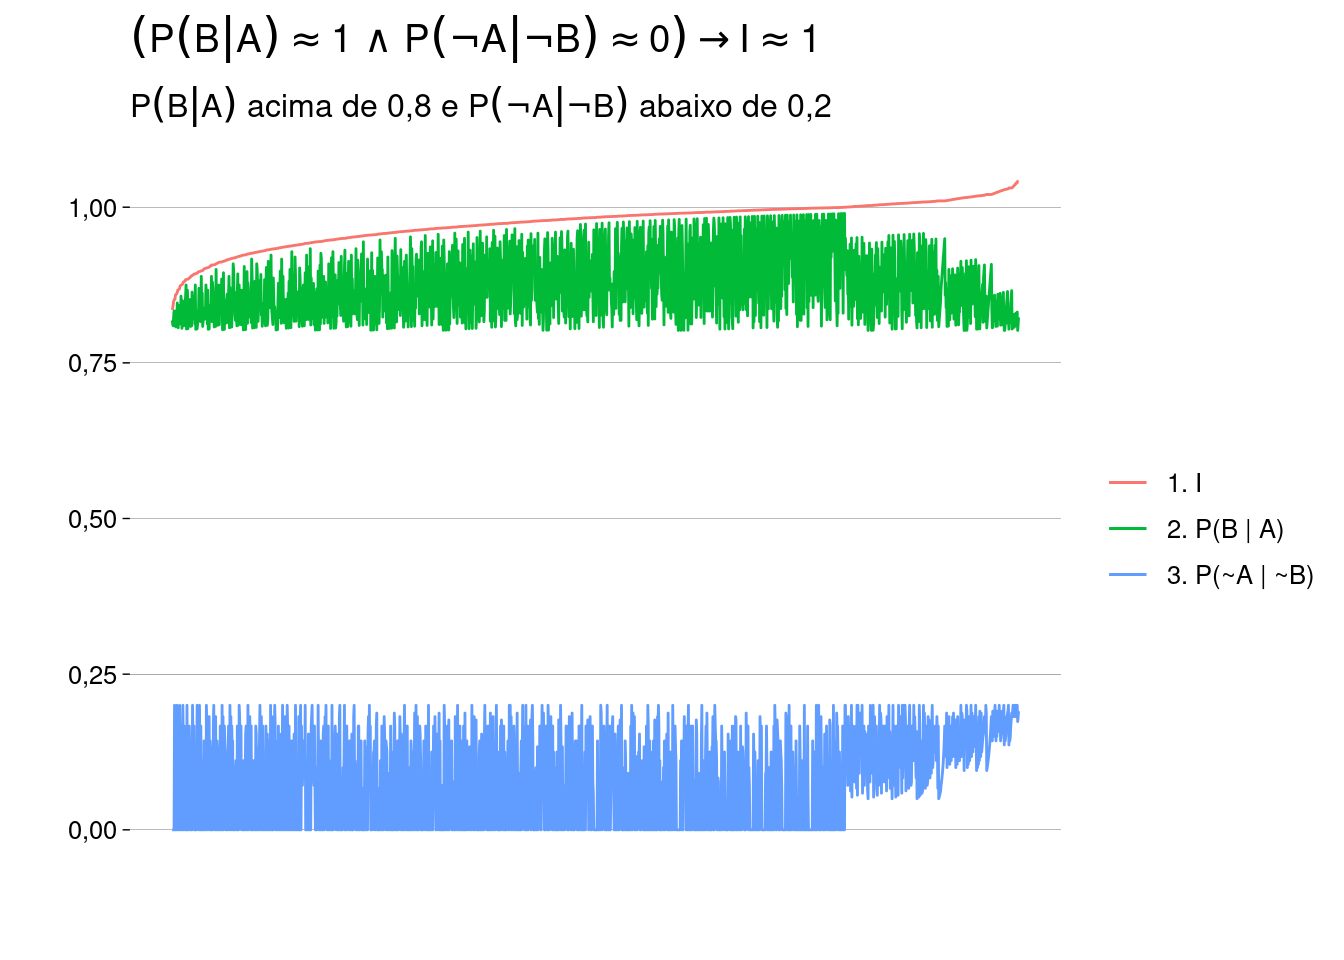
\includegraphics[width=1\linewidth]{_main_files/figure-latex/unnamed-chunk-36-1} \end{center}

\hypertarget{section-15}{%
\subsection*{22}\label{section-15}}
\addcontentsline{toc}{subsection}{22}

\begin{rmdbox}

Este problema foi proposto pela primeira vez por Lewis Carroll em 1893.

\begin{itemize}
\item
  Uma bolsa contém uma bola, que é ou azul, ou verde, com probabilidades iguais.
\item
  Uma bola verde é colocada na bolsa; agora, há $2$ bolas na bolsa.
\item
  Uma bola é retirada da bolsa ao acaso.
\item
  A bola retirada é verde.
\item
  Qual é a probabilidade de que a bola que sobrou na bolsa seja verde?
\end{itemize}

\end{rmdbox}

\begin{itemize}
\item
  Antes de mais nada, vamos definir os eventos:

  \[
  \begin{aligned}
    O &= \text{bola original é verde} \\
    R &= \text{bola retirada é verde} \\
    S &= \text{bola que sobrou é verde}
  \end{aligned}
  \]
\item
  O importante é perceber que o enunciado diz que o evento $R$ aconteceu, mas as probabilidades devem ser calculadas pensando em todos os resultados possíveis, {\hl{antes de o experimento acontecer.}}
\item
  Ou seja, em vez de tomar $P(R) = 1$ --- {\hl{o que seria errado}} --- vamos calcular $P(S \mid R)$: a probabilidade de que a bola que sobrou seja verde, {\hl{sabendo que a bola retirada foi verde.}}
\item
  Começamos com a lei da probabilidade total, condicionando aos dois casos possíveis:

  \[
  \begin{aligned}
  P(S \mid R) &= 
  \underbrace{P(S \mid R, O) \cdot P(O \mid R)}_{\text{caso 1: bola original verde}} 
  \;+\;
  \underbrace{P(S \mid R, \neg O) \cdot P(\neg O \mid R)}_{\text{caso 2: bola original azul}}  
  \end{aligned}
  \]
\item
  No caso $1$:

  \[
  \begin{aligned}
  P(S \mid R, O) \cdot P(O \mid R) 
  &= 1 \cdot P(O \mid R) \\
  &= P(O \mid R)
  \end{aligned}
  \]
\item
  No caso $2$:

  \[
  \begin{aligned}
  P(S \mid R, \neg O) \cdot P(\neg O \mid R) 
  &= 0 \cdot P(\neg O \mid R) \\
  &= 0
  \end{aligned} 
  \]

  Isto faz sentido: {\hl{se a bola original era azul, não há como a bola que sobrou ser verde.}}
\item
  Só precisamos calcular a probabilidade do caso $1$, que é $P(O \mid R)$. Vamos usar Bayes:

  \[
  \begin{aligned}
  P(O \mid R) 
  &= \frac{P(R \mid O) \cdot P(O)}{P(R)} \\
  &= \frac{1 \cdot 1/2}{P(R)}
  \end{aligned}
  \]
\item
  Para calcular $P(R)$, lei da probabilidade total de novo, condicionando sobre a bola original:

  \[
  \begin{aligned}
  P(R) 
  &= P(R \mid O) \cdot P(O) + P(R \mid \neg O) \cdot P(\neg O) \\
  &= 1 \cdot 1/2 + 1/2 \cdot 1/2 \\
  &= 3/4
  \end{aligned}
  \]
\item
  Chegamos a

  \[
  \begin{aligned}
  P(O \mid R) 
  &= \frac{P(R \mid O) \cdot P(O)}{P(R)} \\
  &= \frac{1 \cdot 1/2}{P(R)} \\
  &= \frac{1/2}{3/4} \\
  &= \frac{2}{3}
  \end{aligned}
  \]
\item
  Outra maneira de calcular $P(S \mid R)$ seria aplicar Bayes primeiro:

  \[
  P(S \mid R) = \frac{P(R \mid S) \cdot P(S)}{P(R)}
  \]

  mas as probabilidades do numerador são mais difíceis de calcular! Teríamos que usar a lei da probabilidade total duas vezes para o numerador (além de uma vez para o denominador).
\end{itemize}

\hypertarget{section-16}{%
\subsection*{29}\label{section-16}}
\addcontentsline{toc}{subsection}{29}

\begin{rmdbox}

Uma família tem $2$ crias.

Cada cria tem a mesma probabilidade de ser menino ou menina, e os sexos delas são independentes.

Cada cria tem a característica $C$ com probabilidade $p$, independentemente uma da outra e do sexo.

Mostre que a probabilidade de serem {\hl{duas meninas}}, dado que {\hl{pelo menos uma das crias é uma menina com a característica $C$}}, é

\[
\frac{2 - p}{4 - p}
\]

Observe:

\begin{itemize}
\item
  Se $p = 1$, então a probabilidade é $1/3$, como no exemplo 2.2.5.
\item
  Se $p \to 0$, então a probabilidade tende a $1/2$ pela esquerda, como no exemplo 2.2.7.
\end{itemize}

\end{rmdbox}

\begin{itemize}
\item
  Eventos:

  \[
  \begin{aligned}
  AA &= \text{As duas são meninas} \\
  AC &= \text{Pelo menos uma é menina e tem } C
  \end{aligned}
  \]
\item
  Vamos usar Bayes:

  \[
  P(AA \mid AC) = \frac{P(AC \mid AA) \cdot P(AA)}{P(AC)}
  \]
\item
  A probabilidade de ambas serem meninas é

  \[
  P(AA) = 1/4
  \]
\item
  A probabilidade $P(AC)$ de pelo menos uma ser menina e ter $C$ é a soma das probabilidades de

  \begin{itemize}
  \item
    Ambas serem meninas, ambas terem $C$: $\frac14 \cdot p^2$.
  \item
    Ambas serem meninas, só uma ter $C$ (a primeira ou a segunda): $2 \cdot \frac14 \cdot p \cdot (1 - p)$.
  \item
    Uma ser menina com $C$, a outra ser menino (com ou sem $C$): $\frac12 \cdot p$.
  \item
    Logo,
    \[
    P(AC) = \frac{p \cdot (4 - p)}{4}
    \]
  \end{itemize}
\item
  A probabilidade $P(AC \mid AA)$ de uma ser menina com $C$, dado que ambas são meninas, é

  \[
  \begin{aligned}
  P(AC \mid AA) &= 1 - (1 - p)^2 \\
  &= p \cdot (2 - p)
  \end{aligned}
  \]
\item
  Juntando tudo:

  \[
  \begin{aligned}
  P(AA \mid AC) 
  &= \frac{P(AC \mid AA) P(AA)}{P(AC)} \\
  &= \frac
    {p \cdot (2 - p) \cdot 1/4}
    {p \cdot (4 - p) \cdot 1/4} \\
  &= \frac{2 - p}{4 - p}
  \end{aligned}
  \]
\item
  Um gráfico:

  \begin{center}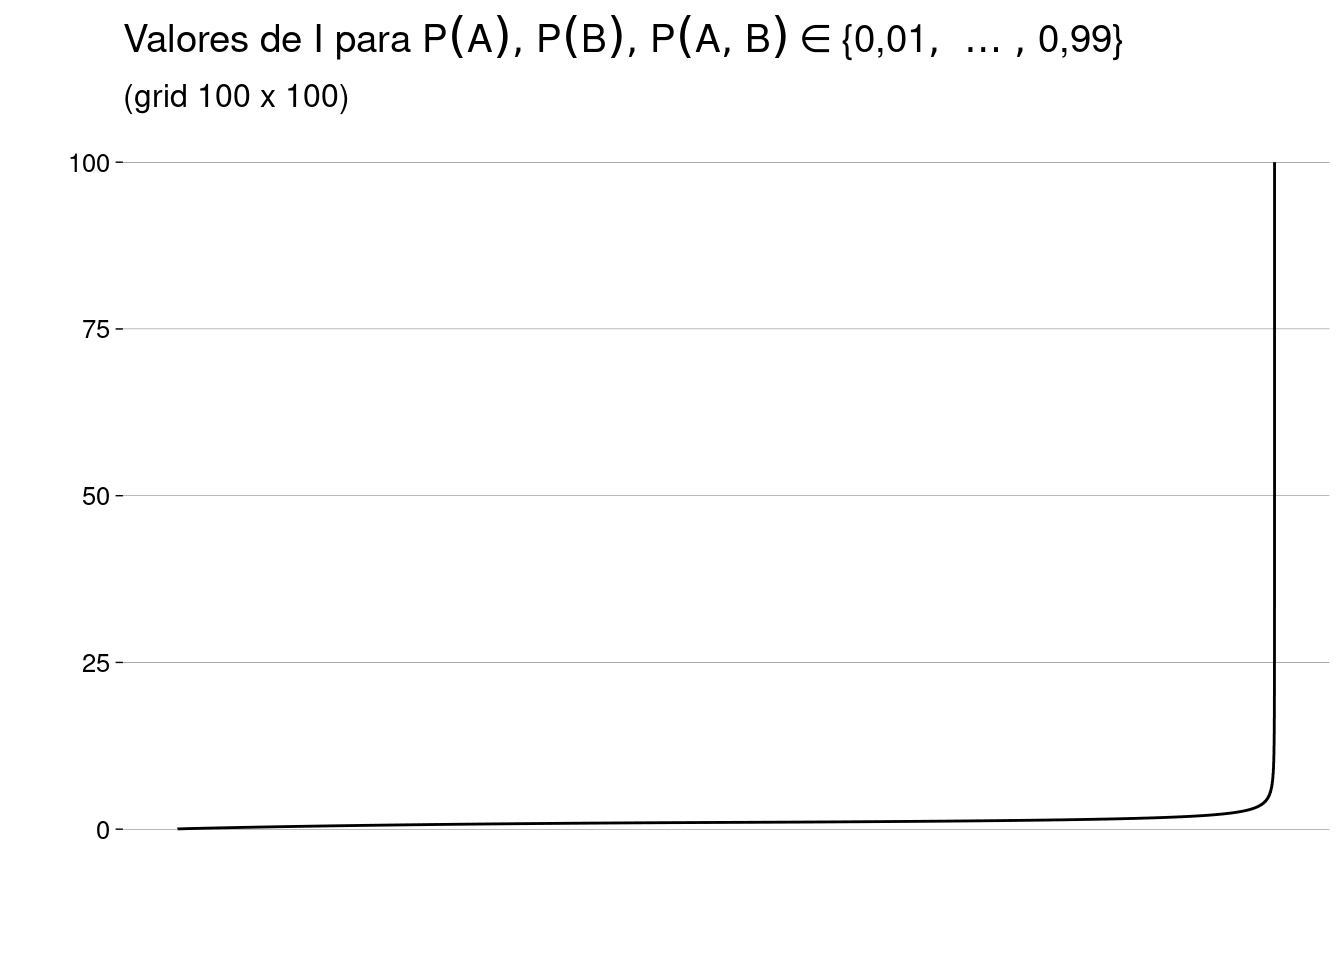
\includegraphics[width=1\linewidth]{_main_files/figure-latex/unnamed-chunk-37-1} \end{center}
\end{itemize}

\hypertarget{probabilidade-condicional-continuauxe7uxe3o}{%
\chapter*{05: Probabilidade condicional (continuação)}\label{probabilidade-condicional-continuauxe7uxe3o}}
\addcontentsline{toc}{chapter}{05: Probabilidade condicional (continuação)}

\hypertarget{vuxeddeo-4}{%
\section*{Vídeo}\label{vuxeddeo-4}}
\addcontentsline{toc}{section}{Vídeo}

\begin{center} \url{https://youtu.be/JzDvVgNDxo8} \end{center}

\hypertarget{exercuxedcios-do-livro-cap.-2-1}{%
\section*{Exercícios do livro (cap. 2)}\label{exercuxedcios-do-livro-cap.-2-1}}
\addcontentsline{toc}{section}{Exercícios do livro (cap. 2)}

\hypertarget{filho-mais-velho}{%
\subsection*{30. Filho mais velho}\label{filho-mais-velho}}
\addcontentsline{toc}{subsection}{30. Filho mais velho}

\begin{rmdbox}

Uma família tem $3$ filhos: $A$, $B$ e $C$.

\begin{enumerate}
\def\labelenumi{\alph{enumi}.}
\tightlist
\item
  O evento ``$A$ é mais velho que $B$'' é independente de ``$A$ é mais velho que $C$''?
\end{enumerate}

\end{rmdbox}

\begin{itemize}
\item
  Intuitivamente:

  Não, pois $A$ ser mais velho que $B$ torna mais provável que $A$ seja mais velho que $C$.
\end{itemize}

\begin{rmdbox}

\begin{enumerate}
\def\labelenumi{\alph{enumi}.}
\setcounter{enumi}{1}
\tightlist
\item
  Qual a probabilidade de que $A$ é mais velho que $B$, dado que $A$ é mais velho que $C$?
\end{enumerate}

\end{rmdbox}

\begin{itemize}
\item
  Queremos achar $P(A > B \mid A > C)$.
\item
  Esta probabilidade é igual a

  \[
  \frac{P(A > B,  A > C)}{P(A > C)}
  \]
\item
  O numerador é a probabilidade de $A$ ser o mais velho.
\item
  Se todas as $6$ ordens de nascimento tiverem a mesma probabilidade,

  \[
  P(A > B,  A > C) = 2/6 = 1/3
  \]
\item
  O denominador é

  \[
  P(A > C) = 3/6 = 1/2
  \]
\item
  Daí, $P(A > B \mid A > C) = \frac{1/3}{1/2} = \frac23$.
\item
  De fato, a probabilidade {\hl{condicional}} $P(A > B \mid A > C) = 2/3$ é {\hl{maior}} do que a probabilidade {\hl{não-condicional}} $P(A > B) = 1/2$.
\end{itemize}

\hypertarget{auto-independuxeancia}{%
\subsection*{31. Auto-independência?}\label{auto-independuxeancia}}
\addcontentsline{toc}{subsection}{31. Auto-independência?}

\begin{rmdbox}
Um evento pode ser independente de si mesmo?

\end{rmdbox}

\begin{itemize}
\item
  Chamando este evento de $A$, é preciso que

  \[
  P(A \cap A) = P(A) = P(A) \cdot P(A)
  \]
\item
  Isto só é possível se $P(A) = 0$ ou se $P(A) = 1$.
\end{itemize}

\hypertarget{dados-de-efron}{%
\subsection*{32. Dados de Efron}\label{dados-de-efron}}
\addcontentsline{toc}{subsection}{32. Dados de Efron}

\begin{rmdbox}

Considere $4$ dados não-padrão (\emph{dados de Efron}), cujos lados são rotulados da seguinte forma (cada lado tem a mesma probabilidade):

\[
\begin{aligned}
  A &: 4, 4, 4, 4, 0, 0 \\
  B &: 3, 3, 3, 3, 3, 3 \\
  C &: 6, 6, 2, 2, 2, 2 \\
  D &: 5, 5, 5, 1, 1, 1
\end{aligned}
\]

Cada dado é lançado uma vez. Cada letra representa o resultado do dado correspondente.

\begin{enumerate}
\def\labelenumi{\alph{enumi}.}
\tightlist
\item
  Ache $P(A > B)$, $P(B > C)$, $P(C > D)$, e $P(D > A)$.
\end{enumerate}

\end{rmdbox}

\begin{itemize}
\item
  Eventos equivalentes:

  \[
  \begin{aligned}
    A > B &\iff A = 4 \\
    B > C &\iff C = 2 \\
    C > D &\iff C = 6 \cup (C = 2 \cap D = 1) \\
    D > A & \iff D = 5 \cup (D = 1\cap A = 0)
  \end{aligned}
  \]
\item
  $P(A > B) = 2/3$.
\item
  $P(B > C) = 2/3$.
\item
  $P(C > D) = 1/3 + 2/3 \cdot 1/2 = 2/3$.
\item
  $P(D > A) = 1/2 + 1/2 \cdot 2/3 = 2/3$.
\end{itemize}

\begin{rmdbox}

\begin{enumerate}
\def\labelenumi{\alph{enumi}.}
\setcounter{enumi}{1}
\item
  O evento $A > B$ é independente de $B > C$?

  O evento $B > C$ é independente de $C > D$?
\end{enumerate}

\end{rmdbox}

\begin{itemize}
\item
  Sim:

  \[
  \begin{aligned}
  P(A > B \cap B > C) &= P(A = 4) \cdot P(C = 2) \\
  &= P(A > B) \cdot P(B > C)
  \end{aligned}
  \]

  Intuitivamente: como o resultado de $B$ não importa para $A > B$ nem para $B > C$, os eventos são independentes.
\item
  Não:

  \[
  \begin{aligned}
    P(B > C \cap C > D) 
    &= P(C = 2 \cap [C = 6 \cup (C = 2 \cap D = 1)]) \\
    &= P((C = 2 \cap C = 6) \cup (C = 2 \cap D = 1)) \\
    &= P(C = 2 \cap D = 1) \\
    &= 2/3 \cdot 1/2 \\
    &= 1/3
  \end{aligned}
  \]

  mas

  \[
  P(B > C) \cdot P(C > D) = 4/9
  \]
\end{itemize}

\hypertarget{amigos}{%
\subsection*{33. Amigos de Alice e Bob}\label{amigos}}
\addcontentsline{toc}{subsection}{33. Amigos de Alice e Bob}

\begin{rmdbox}

\begin{itemize}
\item
  Alice, Bob, e mais $100$ pessoas vivem em uma cidade.
\item
  $C$ é o conjunto das outras $100$ pessoas.
\item
  $A \subseteq C$ é o conjunto de amigos de Alice.
\item
  $B \subseteq C$ é o conjunto de amigos de Bob.
\item
  Para cada pessoa em $C$, a probabilidade de Alice ser amiga da pessoa é $1/2$.
\item
  Idem para Bob.
\item
  As amizades são independentes.
\end{itemize}

\end{rmdbox}

\begin{rmdbox}

\begin{enumerate}
\def\labelenumi{\alph{enumi}.}
\tightlist
\item
  Seja $D \subseteq C$. Achar $P(A = D)$.
\end{enumerate}

\end{rmdbox}

\begin{itemize}
\item
  Para cada $x \in C$:

  \begin{enumerate}
  \def\labelenumi{\arabic{enumi}.}
  \item
    $x \in A \land x \in D$, com probabilidade $\frac12 \cdot \frac{|D|}{|C|}$,

    ou (exclusivo)
  \item
    $x \not\in A \land x \not\in D$, com probabilidade $\frac12 \cdot \left(1 - \frac{|D|}{|C|}\right)$
  \end{enumerate}
\item
  Somando as probabilidades dos casos, para cada $x \in C$, a probabilidade de $x$ estar em $A$ e em $D$, ou de $x$ não estar nem em $A$, nem em $D$, é

  \[
  \frac12 \cdot \frac{|D|}{|C|} + \frac12 \cdot \left(1 - \frac{|D|}{|C|}\right) = \frac12
  \]
\item
  A probabilidade de $A = D$ é a probabilidade de, para todo $x \in C$, acontecer de $x \in A \land x \in D$ ou $x \in A \land x \in D$. Como os eventos são independentes, temos

  \[
  P(A = D) = \frac1{2^{|C|}}
  \]
\item
  Vamos simular a situação. Estamos supondo que os elementos de $D$ são escolhidos segundo uma amostragem simples uniforme, sem reposição. \protect\hyperlink{amostra}{Veja explicações mais detalhadas abaixo}.

\hypertarget{simular-amigos}{%
\label{simular-amigos}}%
\begin{Shaded}
\begin{Highlighting}[]
\NormalTok{simular }\OtherTok{\textless{}{-}} \ControlFlowTok{function}\NormalTok{(p, n) \{}

\NormalTok{  A }\OtherTok{\textless{}{-}}\NormalTok{ (}\DecValTok{1}\SpecialCharTok{:}\NormalTok{n)[}\FunctionTok{runif}\NormalTok{(n) }\SpecialCharTok{\textless{}=}\NormalTok{ p]}
\NormalTok{  D }\OtherTok{\textless{}{-}}\NormalTok{ (}\DecValTok{1}\SpecialCharTok{:}\NormalTok{n)[}\FunctionTok{runif}\NormalTok{(n) }\SpecialCharTok{\textless{}=} \DecValTok{1}\SpecialCharTok{/}\DecValTok{2}\NormalTok{]}

  \ControlFlowTok{if}\NormalTok{ (}\FunctionTok{length}\NormalTok{(A) }\SpecialCharTok{!=} \FunctionTok{length}\NormalTok{(D)) \{}
    \ConstantTok{FALSE}
\NormalTok{  \} }\ControlFlowTok{else}\NormalTok{ \{}
    \FunctionTok{all}\NormalTok{(A }\SpecialCharTok{==}\NormalTok{ D)}
\NormalTok{  \}}

\NormalTok{\}}
\end{Highlighting}
\end{Shaded}
\item
  Para as probabilidades não ficarem tão pequenas, vamos usar um universo $C$ com $10$ elementos apenas:

\hypertarget{simular-com-p}{%
\label{simular-com-p}}%
\begin{Shaded}
\begin{Highlighting}[]
\NormalTok{p }\OtherTok{\textless{}{-}} \DecValTok{1}\SpecialCharTok{/}\DecValTok{2}
\NormalTok{n }\OtherTok{\textless{}{-}} \DecValTok{10}
\NormalTok{nsims }\OtherTok{\textless{}{-}} \FloatTok{1e6}

\NormalTok{resultado }\OtherTok{\textless{}{-}} \FunctionTok{mean}\NormalTok{(}
  \DecValTok{1}\SpecialCharTok{:}\NormalTok{nsims }\SpecialCharTok{\%\textgreater{}\%} 
    \FunctionTok{map\_lgl}\NormalTok{(}\SpecialCharTok{\textasciitilde{}}\FunctionTok{simular}\NormalTok{(p, n))}
\NormalTok{)}

\FunctionTok{cat}\NormalTok{(}\StringTok{\textquotesingle{}P(A = D) simulado = \textquotesingle{}}\NormalTok{, resultado)}
\end{Highlighting}
\end{Shaded}

\begin{verbatim}
## P(A = D) simulado =  0,000991
\end{verbatim}

\hypertarget{simular-com-p}{%
\label{simular-com-p}}%
\begin{Shaded}
\begin{Highlighting}[]
\FunctionTok{cat}\NormalTok{(}\StringTok{\textquotesingle{}P(A = D) teórico  = \textquotesingle{}}\NormalTok{, }\DecValTok{1}\SpecialCharTok{/}\DecValTok{2}\SpecialCharTok{\^{}}\NormalTok{n)}
\end{Highlighting}
\end{Shaded}

\begin{verbatim}
## P(A = D) teórico  =  0,0009765625
\end{verbatim}
\item
  E se $p \neq 1/2$?
\item
  \protect\hyperlink{amostra}{Como explicado abaixo}, a probabilidade de um $x \in C$ pertencer a $D$ (supondo que $D$ é obtido por amostragem simples) é $1/2$.
\item
  Então, Para cada $x \in C$:

  \begin{enumerate}
  \def\labelenumi{\arabic{enumi}.}
  \item
    $x \in A \land x \in D$, com probabilidade $p/2$,

    ou (exclusivo)
  \item
    $x \not\in A \land x \not\in D$, com probabilidade $(1 - p)/2$
  \end{enumerate}
\item
  Somando as probabilidades dos casos, para cada $x \in C$, a probabilidade de $x$ estar em $A$ e em $D$, ou de $x$ não estar nem em $A$, nem em $D$, é, de novo, $1/2$.
\item
  Logo, $P(A = D) = 1/ 2^{|C|}$ novamente.
\item
  Ou seja, {\hl{o resultado vale para qualquer valor de $p$.}} Altere o valor de $p$ no \protect\hyperlink{simular-com-p}{código da simulação acima} para verificar.
\end{itemize}

\begin{rmdbox}

\begin{enumerate}
\def\labelenumi{\alph{enumi}.}
\setcounter{enumi}{1}
\tightlist
\item
  Achar $P(A \subseteq B)$
\end{enumerate}

\end{rmdbox}

\begin{itemize}
\item
  Para cada $x \in A$, a probabilidade de $x \in B$ é $1/2$.
\item
  Logo, $P(A \subseteq B) = 1 / 2^{|A|}$.
\end{itemize}

\begin{rmdbox}

\begin{enumerate}
\def\labelenumi{\alph{enumi}.}
\setcounter{enumi}{2}
\tightlist
\item
  Achar $P(A \cup B) = C$.
\end{enumerate}

\end{rmdbox}

\begin{itemize}
\item
  Para cada $x \in C$,

  \[
  \begin{aligned}
  P(x \in A \cup B) 
  &= P(x \in A) + P(x \in B) - P(x \in A \cap B) \\
  &= 1/2 + 1/2 - 1/4 \\
  &= 3/4
  \end{aligned}
  \]
\item
  Logo, $P(A \cup B = C) = (3/4)^{|C|}$
\end{itemize}

\hypertarget{amostra}{%
\subsection*{Extra: amostragem simples}\label{amostra}}
\addcontentsline{toc}{subsection}{Extra: amostragem simples}

\begin{itemize}
\item
  \protect\hyperlink{amigos}{Na resolução acima}, usamos a igualdade

  \[
  P(x \in D) = \frac{|D|}{n}
  \]

  para representar a probabilidade de que um elemento qualquer de um universo com $n$ elementos pertença a um {\hl{conjunto $D$ fixo}}.
\item
  Mas e quando não sabemos qual é o conjunto $D$, nem qual o seu tamanho?
\item
  Neste caso, precisamos supor algo sobre a distribuição dos subconjuntos.
\item
  O mais comum é supor que {\hl{cada um dos $2^n$ subconjuntos tem a mesma probabilidade de ser o resultado da amostragem.}}
\item
  Com esta suposição, como calculamos $P(x \in D)$?
\item
  Vamos condicionar ao tamanho do conjunto $D$ e marginalizar:

  \[
  P(x \in D) = \sum_{k = 0}^{n} P(x \in D \mid |D| = k) \cdot P(|D| = k)
  \]
\item
  Calculando a primeira probabilidade dentro do somatório:

  \[
  \begin{aligned}
  P(x \in D \mid |D| = k) 
  &= \frac{\binom{n - 1}{k - 1}}{\binom n k} \\
  &= \frac k n
  \end{aligned}
  \]

  Na primeira linha, o numerador é a quantidade de subconjuntos de $k$ elementos que contêm $x$ (basta escolher os outros $k - 1$ elementos dentre os $n - 1$ outros elementos do universo); o denominador é o total de subconjuntos de $k$ elementos.

  Perceba que {\hl{aqui usamos a suposição de que todos os subconjuntos têm a mesma probabilidade de ser amostrados}}.

  Perceba também que, como antes, esta probabilidade é igual a $\frac{|D|}{n}$.
\item
  Calculando a segunda probabilidade dentro do somatório:

  \[
  \begin{aligned}
  P(|D| = k)
  &= \frac{\binom{n}{k}}{2^n}
  \end{aligned}
  \]

  De novo, usando a suposição de que todos os subconjuntos são equiprováveis, temos a quantidade de subconjuntos de $k$ elementos sobre o total de subconjuntos.
\item
  Juntando tudo:

  \[
  \begin{aligned}
  P(x \in D) 
  &= \sum_{k = 0}^{n} P(x \in D \mid |D| = k) \cdot P(|D| = k) \\
  &= \sum_{k = 0}^{n} \frac 1 {2^n} \binom n k \frac k n \\
  &= \frac 1 {2^n} \sum_{k = 0}^{n} \binom{n - 1}{k - 1} \\
  &= \frac 1 {2^n} \cdot 2^{n - 1} \\
  &= \frac 1 2
  \end{aligned}
  \]

  \begin{rmdimportant}
  Fazer amostragem uniforme significa que todos os subconjuntos são equiprováveis, {\hl{ou, equivalentemente, que cada elemento do universo tem $50\%$ de chance de estar na amostra.}}

  \end{rmdimportant}
\item
  Por isso, \protect\hyperlink{simular-amigos}{na simulação}, geramos o conjunto $D$ com o comando

  \texttt{D\ \textless{}-\ (1:n){[}runif(n)\ \textless{}=\ 1/2{]}}
\end{itemize}

\hypertarget{xadrez}{%
\subsection*{35. Xadrez}\label{xadrez}}
\addcontentsline{toc}{subsection}{35. Xadrez}

\begin{rmdbox}

\begin{itemize}
\item
  Você vai jogar $2$ partidas de xadrez contra um adversário desconhecido.
\item
  O nível do seu adversário pode ser novato, intermediário, ou avançado, com probabilidades iguais.
\item
  As probabilidades de você vencer uma partida são, dependendo do nível do adversário, respectivamente, $90\%$, $50\%$, e $30\%$.
\end{itemize}

\begin{enumerate}
\def\labelenumi{\alph{enumi}.}
\item
  Qual a probabilidade de você vencer a primeira partida?
\item
  Parabéns, você venceu a primeira partida. Dada esta informação, qual a probabilidade de que você também vença a segunda partida (suponha que, {\hl{dado o nível do seu adversário}}, os resultados das partidas são independentes)?
\item
  Explique a diferença entre

  \begin{enumerate}
  \def\labelenumii{\arabic{enumii}.}
  \item
    supor que os resultados das partidas são independentes, e
  \item
    supor que os resultados das partidas são independentes, dado o nível do seu adversário.
  \end{enumerate}

  Qual destas suposições parece mais razoável? Por quê?
\end{enumerate}

\end{rmdbox}

\begin{itemize}
\item
  Antes de mais nada, vamos definir os eventos:

  \[
  \begin{aligned}
    N &= \text{o adversário é novato} \\
    I &= \text{o adversário é intermediário} \\
    A &= \text{o adversário é avançado} \\
    V_1 &= \text{você vence a primeira partida} \\
    V_2 &= \text{você vence a segunda partida} 
  \end{aligned}
  \]
\item
  O enunciado dá as probabilidades

  \[
  \begin{aligned}
  P(N) &= 1/3 \\
  P(I) &= 1/3 \\
  P(A) &= 1/3 \\
  P(V_1 \mid N) &= 9/10 \\
  P(V_1 \mid I) &= 5/10 \\
  P(V_1 \mid A) &= 3/10
  \end{aligned}
  \]
\item
  Para resolver (a), basta usar probabilidade total, condicionando sobre o nível do adversário:

  \[
  \begin{aligned}
  P(V_1) 
  &= 
  P(V_1 \mid N) \cdot P(N) \;+\;
  P(V_1 \mid I) \cdot P(I) \;+\;
  P(V_1 \mid A) \cdot P(A)
  \\
  &= 
  \frac{9}{10} \cdot \frac{1}{3} + 
  \frac{5}{10} \cdot \frac{1}{3} + 
  \frac{3}{10} \cdot \frac{1}{3} \\
  &= 
  \frac{1}{3} \cdot \left(
  \frac{9}{10} + 
  \frac{5}{10} + 
  \frac{3}{10} \right) \\
  &=
  \frac{17}{30}
  \end{aligned}
  \]

  Faz sentido. Como as probabilidades dos níveis possíveis do adversário são iguais, a probabilidade de vencer é {\hl{a média aritmética}} das probabilidades de vencer contra cada nível.

  Se as probabilidades dos níveis do adversário fossem diferentes, seria a {\hl{média ponderada.}}
\item
  Para (b), queremos calcular $P(V_2 \mid V_1)$.

  Dizer que $V_1$ e $V_2$ são independentes {\hl{dado o nível do adversário}} é dizer

  \[
  P(V_2 \mid V_1, N) = P(V_1 \mid V_2, N) = P(V_2 \mid N) = P(V_1 \mid N)
  \]

  e analogamente para probabilidades condicionadas a $I$ e a $A$.

  Ou seja, dado um nível específico do adversário, saber que $V_1$ ocorreu não altera a probabilidade de $V_2$ ocorrer, e vice-versa.

  Vamos calcular $P(V_2 \mid V_1)$ usando probabilidade total, condicionando ao nível:

  \[
  \begin{aligned}
  \underbrace{P(V_2 \mid V_1, N) \cdot P(N \mid V_1)}_{\text{novato}}
  \;+\;
  \underbrace{P(V_2 \mid V_1, I) \cdot P(I \mid V_1)}_{\text{intermediário}}
  \;+\;
  \underbrace{P(V_2 \mid V_1, A) \cdot P(A \mid V_1)}_{\text{avançado}}
  \end{aligned}
  \]

  Para o lado esquerdo de cada produto, a independência condicional diz que

  \begin{alignat*}{3}
  P(V_2 \mid V_1, N) &= P(V_1 \mid N) &= 9/10 \\
  P(V_2 \mid V_1, I) &= P(V_1 \mid I) &= 5/10 \\
  P(V_2 \mid V_1, A) &= P(V_1 \mid A) &= 3/10
  \end{alignat*}

  Para o lado direito de cada produto, usamos Bayes. Todas as probabilidades envolvidas já foram calculadas.

  Novato:

  \[
  \begin{aligned}
  P(N \mid V_1) 
  &=
  \frac{P(V_1 \mid N) \cdot P(N)}{P(V_1)}
  \\
  &= \frac{9/10 \cdot 1/3}{17/30}
  \\
  &= \frac{9}{17}
  \end{aligned}
  \]

  Intermediário:

  \[
  \begin{aligned}
  P(I \mid V_1) 
  &=
  \frac{P(V_1 \mid I) \cdot P(I)}{P(V_1)}
  \\
  &= \frac{5/10 \cdot 1/3}{17/30}
  \\
  &= \frac{5}{17}
  \end{aligned}
  \]

  Avançado:

  \[
  \begin{aligned}
  P(A \mid V_1) 
  &=
  \frac{P(V_1 \mid A) \cdot P(A)}{P(V_1)}
  \\
  &= \frac{3/10 \cdot 1/3}{17/30}
  \\
  &= \frac{3}{17}
  \end{aligned}
  \]

  A resposta final é

  \[
  \frac{9}{10} \cdot \frac{9}{17} \;+\;
  \frac{5}{10} \cdot \frac{5}{17} \;+\;
  \frac{3}{10} \cdot \frac{3}{17}
  \;=\;
  \frac{23}{34}
  \]
\item
  Para responder (c):

  Dizer que $V_1$ e $V_2$ são {\hl{incondicionalmente}} independentes seria dizer que

  \[
  P(V_2 \mid V_1) = P(V_2)
  \]

  Ainda mais, como o nível do adversário não muda de uma partida para outra, teríamos também

  \[
  P(V_2) = P(V_1)
  \]

  Ou seja, cada partida seria uma prova de Bernoulli com a mesma probabilidade de sucesso.

  Considerando independência {\hl{condicional}}, saber que vencemos a primeira partida nos dá informação sobre o nível do adversário, e esta informação é considerada para calcular a probabilidade de vencer a segunda partida.

  De fato, usando independência condicional, temos

  \[
  P(V_1) \approx 0{,}57
  \]

  e

  \[
  P(V_2 \mid V_1) \approx 0{,}68
  \]
\end{itemize}

\hypertarget{paradoxo-de-berkson}{%
\subsection*{\texorpdfstring{36. \href{https://en.wikipedia.org/wiki/Berkson\%27s_paradox}{Paradoxo de Berkson}}{36. Paradoxo de Berkson}}\label{paradoxo-de-berkson}}
\addcontentsline{toc}{subsection}{36. \href{https://en.wikipedia.org/wiki/Berkson\%27s_paradox}{Paradoxo de Berkson}}

\begin{rmdbox}
{\hl{Se}}

\begin{itemize}
\item
  $A$ e $B$ são independentes, e
\item
  $P(A \cap B) > 0$, e
\item
  $P(A \cup B) < 1$, e
\item
  $C = A \cup B$
\end{itemize}

{\hl{então}} $A$ e $B$ são condicionalmente dependentes, dado $C$, com

\[
P(A \mid B, C) < P(A \mid C)
\]

Exemplo: universidade admite candidatos que são bons jogadores de basquete ($A$) ou que são bons em Matemática ($B$) --- {\hl{supondo que estes são eventos independentes, o que é meio duvidoso}}.\footnote{Na verdade, em vez de independência entre $A$ e $B$, basta que um evento atrapalhe o outro para termos o paradoxo. Em termos da \protect\hyperlink{i}{nossa medida de independência $I$}, basta $0< I < 1$.}

\end{rmdbox}

\begin{itemize}
\item
  De $P(A \cap B) > 0$, temos que $P(A) > 0$ e que $P(B) > 0$.
\item
  Daí, $P(C) = P(A \cup B) > 0$.
\item
  Para o lado esquerdo:

  \[
  \begin{aligned}
  P(A \mid B, C) 
  &= \frac{P(A \cap B \cap C)}{P(B \cap C)} \\
  &= \frac{P(A \cap B)}{P(B)} \\
  &= \frac{P(A)P(B)}{P(B)} \\
  &= P(A)
  \end{aligned}
  \]
\item
  Para o lado direito:

  \[
  \begin{aligned}
  P(A \mid C) 
  &= \frac{P(A \cap C)}{P(C)} \\
  &= \frac{P(A)}{P(C)} \\
  &= \frac{P(A)}{P(A \cup B)} 
  \end{aligned}
  \]
\item
  Como o denominador $P(A \cup B) < 1$, esta probabilidade é maior do que $P(A)$.
\end{itemize}

\hypertarget{doenuxe7as-e-sintoma}{%
\subsection*{37. Doenças e sintoma}\label{doenuxe7as-e-sintoma}}
\addcontentsline{toc}{subsection}{37. Doenças e sintoma}

\begin{rmdbox}

\begin{itemize}
\item
  Quem tem a doença $D_1$ ou a doença $D_2$ (ou ambas) tem o sintoma estranho $W$.
\item
  $D_1$ e $D_2$ são independentes, com $P(D_j) = p_j$, e com $q_j = 1 - p_j$.
\item
  $0 < p_j < 1$.
\item
  Uma pessoa sadia tem o sintoma $W$ com probabilidade $w_0$.
\end{itemize}

\end{rmdbox}

\begin{rmdbox}

\begin{enumerate}
\def\labelenumi{\alph{enumi}.}
\tightlist
\item
  Achar $P(W)$.
\end{enumerate}

\end{rmdbox}

\begin{itemize}
\item
  Por probabilidade total:

  \[
  \begin{aligned}
  P(W) 
  &= P(W \mid D_1 \cup D_2) \cdot P(D_1 \cup D_2) +
  P(W \mid \neg(D_1 \cup D_2)) \cdot P(\neg(D_1 \cup D_2)) \\
  &= 1 \cdot (p_1 + p_2 - p_1p_2) + w_0 \cdot (1 - p_1 - p_2 + p_1p_2) \\
  &= p_1 + p_2 - p_1p_2 + w_0q_1q_2 
  \end{aligned}
  \]
\end{itemize}

\begin{rmdbox}

\begin{enumerate}
\def\labelenumi{\alph{enumi}.}
\setcounter{enumi}{1}
\tightlist
\item
  Achar $P(D_1 \mid W)$, $P(D_2 \mid W)$, e $P(D_1 \cap D_2 \mid W)$.
\end{enumerate}

\end{rmdbox}

\begin{itemize}
\item
  Por Bayes:

  \[
  \begin{aligned}
    P(D_1 \mid W) 
    &= \frac{P(W \mid D_1) \cdot P(D_1)}{P(W)} \\
    &= \frac{1 \cdot p_1}{p_1 + p_2 - p_1p_2 + w_0q_1q_2} \\
    &= \frac{p_1}{p_1 + p_2 - p_1p_2 + w_0q_1q_2}
  \end{aligned}
  \]
\item
  Analogamente,

  \[
  P(D_2 \mid W) = \frac{p_2}{p_1 + p_2 - p_1p_2 + w_0q_1q_2}
  \]
\item
  Finalmente,

  \[
  \begin{aligned}
  P(D_1 \cap D_2 \mid W)
  &= \frac{P(D_1 \cap D_2 \cap W)}{P(W)} \\
  &= \frac{P(D_1 \cap D_2)}{P(W)} & (\text{pois }D_1 \cap D_2 \subseteq W)\\
  &= \frac{p_1p_2}{p_1 + p_2 - p_1p_2 + w_0q_1q_2}
  \end{aligned}
  \]
\end{itemize}

\begin{rmdbox}

\begin{enumerate}
\def\labelenumi{\alph{enumi}.}
\setcounter{enumi}{2}
\tightlist
\item
  $D_1$ e $D_2$ são condicionalmente independentes, dado $W$?
\end{enumerate}

\end{rmdbox}

\begin{itemize}
\item
  Basta verificar se

  \[
  P(D_1 \mid W) \cdot P(D_2 \mid W) = P(D_1 \cap D_2 \mid W)
  \]
\item
  Isto equivale a

  \[
  \frac{p_1p_2}{(p_1 + p_2 - p_1p_2 + w_0q_1q_2)^2} = 
  \frac{p_1p_2}{p_1 + p_2 - p_1p_2 + w_0q_1q_2}
  \]
\item
  {\hl{Esta igualdade só é verdade se}}

  \begin{enumerate}
  \def\labelenumi{\arabic{enumi}.}
  \item
    $w_0 = 0$ e $P(D_1 \cup D_2) = 0$ (o que é proibido pelo enunciado). Ninguém estaria doente, e ninguém teria o sintoma.

    ou
  \item
    $P(D_1 \cup D_2) = 1$. Aqui, todos estariam doentes, e todos teriam o sintoma.
  \end{enumerate}
\item
  Lembramos que

  \[
  w_0 = P(W \mid \neg(D_1 \cup D_2)) = 
  \frac{P(W \cap \neg(D_1 \cup D_2))}{P(\neg(D_1 \cup D_2))}
  \]
\item
  No caso (1) acima, $w_0 = P(W) = 0$, e não faz mais sentido condicionar sobre $W$.
\item
  No caso (2) acima, $P(\neg(D_1 \cup D_2)) = 0$, e a própría definição de $w_0$ deixa de fazer sentido.
\end{itemize}

\begin{rmdbox}

\begin{enumerate}
\def\labelenumi{\alph{enumi}.}
\setcounter{enumi}{3}
\tightlist
\item
  Suponha que $w_0 = 0$. Neste caso, $D_1$ e $D_2$ são condicionalmente independentes, dado $W$?
\end{enumerate}

\end{rmdbox}

\begin{itemize}
\item
  Por causa do discutido no item (c), vamos supor que \[0 < P(D_1 \cup D_2) < 1\] para que possamos condicionar sobre $W$ e para que a definição de $w_0$ faça sentido.
\item
  Como no item (c), verificamos se

  \[
  P(D_1 \mid W) \cdot P(D_2 \mid W) = P(D_1 \cap D_2 \mid W)
  \]
\item
  Que equivale a

  \[
  \frac{p_1p_2}{(p_1 + p_2 - p_1p_2)^2} = 
  \frac{p_1p_2}{p_1 + p_2 - p_1p_2}
  \]
\item
  Isto é impossível, se $0 < P(D_1 \cup D_2) < 1$.
\item
  Intuitivamente, $D_1$ e $D_2$ seriam {\hl{condicionalmente dependentes}}, dado $W$, pois, dado que uma pessoa tem o sintoma $W$, saber que ela não tem a doença $D_1$ imediatamente nos diz que ela tem a doença $D_2$.
\end{itemize}

\begin{rmdnote}
Quando $w_0 = 0$ e $0 < P(D_1 \cup D_2) < 1$, a consequência é que

\[
D_1 \cup D_2 = W
\]
como eventos.

Daí, com as outras condições do enunciado, temos uma instância do \protect\hyperlink{paradoxo-de-berkson}{paradoxo de Berkson}, com $A = D_1$ e $B = D_2$.

\end{rmdnote}

\hypertarget{nauxefve-bayes}{%
\subsection*{38. Naïve Bayes}\label{nauxefve-bayes}}
\addcontentsline{toc}{subsection}{38. Naïve Bayes}

\begin{rmdbox}

\begin{itemize}
\item
  Temos uma lista de $100$ palavras.
\item
  Evento $W_j = {}$ a palavra $j$ aparece no \emph{email}.
\item
  Evento $\text{spam} = {}$ o \emph{email} é \emph{spam}.
\item
  $p = P(\text{spam})$.
\item
  $p_j = P(W_j \mid \text{spam})$.
\item
  $r_j = P(W_j \mid \neg \text{spam})$.
\item
  A \emph{naïveté} do algoritmo consiste nas seguintes suposições --- não-realistas, mas úteis:

  \begin{itemize}
  \item
    Os $W_j$ são condicionalmente independentes, dado $\text{spam}$.
  \item
    Os $W_j$ são condicionalmente independentes, dado $\neg \text{spam}$.
  \end{itemize}
\item
  Um novo \emph{email} é recebido. Contém as palavras $23$, $64$, e $65$, e nenhuma das outras.
\item
  Vamos chamar de $\vec W$ a lista de eventos

  \[
  \begin{array}{l}
  \neg W_1, \ldots, \neg W_{22}, \\
  W_{23},\\ 
  \neg W_{24}, \ldots, \neg W_{63},\\    
  W_{64}, W_{65},\\ 
  \neg W_{66}, \ldots, \neg W_{100}
  \end{array}
  \]
\item
  Calcular $P\left( \text{spam} \;\middle|\; \vec W \right)$.
\end{itemize}

\end{rmdbox}

\begin{itemize}
\item
  Por Bayes:

  \[
  P\left( \text{spam} \;\middle|\; \vec W \right) = 
  \frac{P\left(\vec W \;\middle|\; \text{spam} \right)}
  {P\left( \vec W  \right)}
  \]
\item
  Com a suposição \emph{naïve}, podemos multiplicar as probabilidades condicionais:

  \[
  P\left(\vec W\;\middle|\; \text{spam} \right) =
  p_{23} \cdot p_{64} \cdot p_{65} \cdot
  \!\!\!\!\!\!\!\!\!
  \prod_{
    \begin{array}{c}
    1 \leq j \leq 100. \\
    j \not\in \{ 23, 64, 65 \}
    \end{array}
  }
  \!\!\!\!\!\!\!
  (1 - p_j)
  \]

  {\hl{Vamos chamar este valor de $m$.}}
\item
  Para calcular $P\left( \vec W \right)$, usamos probabilidade total:

  \[
  \begin{aligned}
  P\left( \vec W \right) 
  &= 
    P\left(\vec W \;\middle|\; \text{spam} \right) 
    \cdot P(\text{spam})
    \;+\;
    P\left(\vec W \;\middle|\; \neg\text{spam} \right) 
    \cdot P(\neg\text{spam})
  \\
  &=
    m \cdot p \;+\; m' \cdot (1 - p)
  \end{aligned}
  \]

  onde, de maneira análoga ao cálculo de $m$,

  \[
  m' = 
    r_{23} \cdot r_{64} \cdot r_{65} \cdot
  \!\!\!\!\!\!\!\!\!
  \prod_{
    \begin{array}{c}
    1 \leq j \leq 100. \\
    j \not\in \{ 23, 64, 65 \}
    \end{array}
  }
  \!\!\!\!\!\!\!
  (1 - r_j)
  \]
\item
  O valor procurado é, então,

  \[
  P\left( \text{spam} \;\middle|\; \vec W \right) 
  = 
  \frac{P\left(\vec W \;\middle|\; \text{spam} \right)}
  {P\left( \vec W  \right)}
  = \frac{mp}{mp + m'(1 - p)}
  \]
\end{itemize}

\hypertarget{referuxeancias}{%
\chapter*{Referências}\label{referuxeancias}}
\addcontentsline{toc}{chapter}{Referências}

\hypertarget{refs}{}
\begin{CSLReferences}{0}{1}
\leavevmode\vadjust pre{\hypertarget{ref-devlin-2010-pascal-fermat}{}}%
DEVLIN, K. \href{https://doi.org/10.5951/mt.103.8.0579}{The {P}ascal-{F}ermat Correspondence: How Mathematics Is Really Done}. \textbf{The Mathematics Teacher}, v. 103, n. 8, p. 579--582, abr. 2010.

\leavevmode\vadjust pre{\hypertarget{ref-oliveira-2004-analis}{}}%
OLIVEIRA MORGADO, A. C. DE et al. \textbf{An{á}lise combinat{ó}ria e probabilidade}. Rio de Janeiro: Impa / Vitae, 2004.

\leavevmode\vadjust pre{\hypertarget{ref-paulos-1988-innum}{}}%
PAULOS, J. A. \textbf{\href{http://gen.lib.rus.ec/book/index.php?md5=20A842C0E7EB7F8992EDDA0082E9B76F}{Innumeracy: Mathematical Illiteracy and Its Consequences}}. 1. ed. New York: Hill; Wang, 1988.

\end{CSLReferences}

\end{document}
